% --------------------------------------------------------------------

\chapter[AGN]{Active Galactic Nuclei}
\def\chpname{agn}\label{chp:\chpname}

Chapter editors:
\credit{ohadshemmer},
\credit{tanguita}.

Contributing authors:
\credit{AstroVPK},
\credit{cmp346},
\credit{nielbrandt},
\credit{GordonRichards},
\credit{ScottAnderson},
\credit{mattodowd},
{\it Robert Wagoner}

\section*{Summary}
\addcontentsline{toc}{section}{~~~~~~~~~Summary}

To zeroth order, AGN science with LSST will benefit from the most
uniform cadence in terms of even sampling for each band and uniform sky
coverage while maximizing the area, but excluding the Galactic plane. It
is also expected that any reasonable perturbation to the nominal LSST
observing strategy will not have a major effect on AGN science. While
denser sampling at shorter wavelengths will aid investigations of the
size and structure of the AGN central engine via intrinsic continuum
variability and microlensing, care must be taken not to compromise the
coadded $Y$-band depth which is crucial for detecting the most distant
quasars. Assuming two visits per night, two different bands are
preferred. Science cases related to intrinsic continuum and
broad-emission line variability will benefit from the denser sampling
offered in the DDFs. These fields will provide powerful ``truth tables''
that are crucial for AGN selection algorithms, enable construction of
high-quality power spectral density functions, and enable measurements
of continuum-continuum and line-continuum time lags. The benefits and
tradeoffs with respect to the main survey involve high-quality light
curves but for only a small fraction ($\sim1$\%) of all sources,
preferentially those at lower luminosities. Certain science cases will
benefit greatly from even denser sampling, i.e., $\sim1 -
1000$~d$^{-1}$, of a smaller area, perhaps during the commissioning
phase, as long as the temporal baseline will extend over the ten years
of the project. Another justification to this strategy is the fact that
very few AGNs, or transient AGNs, have been monitored at these
frequencies on such a long baseline, leaving room for discovery.

% --------------------------------------------------------------------

\section{Introduction}
\label{sec:\chpname:intro}

% Introduce, with a very broad brush, this chapter's science projects,
% and why it makes sense for them to be considered together.

The purpose of this chapter is to identify AGN science cases that may be
affected by the LSST observing strategy and to specify the metrics that can be
used to quantify any potential effects. Since the total number of metrics that
can be quantified is quite large, and the potential effects are not likely to be
significant in most cases, the goal of this chapter is to identify potential
``show stoppers'' that may undermine key AGN research areas. For example,
certain perturbations may reduce significantly the number of ``interesting'' AGNs,
such as $z > 6$ quasars, lensed quasars, or transient AGNs. Another example is
photometric reverberation mapping which is one of LSST's greatest potential
advantages for AGN research but is also very sensitive to the cadence; care must
be taken to ensure that the observing strategy does not undermine the ability to
make the best use of this method.

%This chapter discusses the potential effects of the LSST observing
%strategy on AGN science. In short, there appears to be a consensus
%among the AGN and galaxies communities that AGN science will benefit
%from the most uniform cadence in terms of even sampling for each band
%and uniform sky coverage. It is also expected that any reasonable
%perturbation to the nominal LSST observing strategy will not have a major
%effect on AGN science. This chapter attempts to identify all
%the areas of AGN science that may be affected by the observing strategy
%and to point out the metrics that can be used to quantify any potential
%effects. Since the total number of metrics that can be quantified is
%quite large, and the potential effects are not likely to be significant in
%most cases, the goal of this chapter is to identify potential ``show
%stoppers'' that may undermine key AGN research areas. For example, certain
%perturbations may reduce significantly the number of ``interesting'' AGNs,
%such as $z>6$ quasars, lensed quasars, or transient AGNs. Another example
%is photometric reverberation mapping which is one of LSST's greatest
%potential advantages for AGN research but is also very sensitive to the
%cadence; care must be taken to ensure that the observing strategy does
%not undermine the ability to make the best use of this method.

This chapter is organized as follows. Section~\ref{sec:AGNCensus}
describes potential effects the LSST Observing Strategy may have on the
selection of LSST AGNs in the entire survey, hereafter, the AGN
census. Subsamples of this census are then used throughout this chapter for
discussing particular science cases. Section~\ref{sec:AGNContinuum}
discusses potential effects of the Observing Strategy on studying AGN continuum
(or disk) variability. Section~\ref{sec:AGNMicrolensing} describes how the
LSST cadence may affect estimates or constraints on the size and structure of
the AGN central engine from observations of microlensing events.
Section~\ref{sec:AGNFuture} presents science cases that are still being
developed quantitatively, including sampling effects on measurements related
to the broad emission line region in AGNs. Finally,
section~\ref{sec:AGNDiscussion} discusses additional AGN science aspects that
may be affected significantly by the LSST cadence.

Note: Transient AGN and tidal disruption events are discussed in
detail in the transients chapter
(\autoref{chp:transients}), while gravitationally-lensed AGN are
covered in the cosmology chapter (\autoref{sec:lenstimedelays}).


% --------------------------------------------------------------------

% PJM: moved to Future Work while MAF analysis is pending:
% % ====================================================================
%+
% SECTION:
%    AGN_Census.tex
%
% CHAPTER:
%    agn.tex
%
% ELEVATOR PITCH:
%-
% ====================================================================

% \section{AGN Selection and Census}
\section{AGN Selection and Census}\label{sec:AGNCensus}
\def\secname{\chpname:census}\label{sec:\secname}

\credit{ohadshemmer},
\credit{nielbrandt},
\credit{GordonRichards},
\credit{AstroVPK},
\credit{ScottAnderson}

One basic figure of merit for AGN science is the total number of AGNs
discovered in the entire LSST survey, as a function of luminosity and
redshift. The main goal is therefore to adjust the Observing Strategy
in order to maximize this number.
%The primary goal for AGN science is to maximize the discovery of AGN
%with the LSST and construct the largest possible inventory of sources
%spanning the widest possible ranges in the redshift-luminosity parameter
%space. This, in turn, will provide
Doing so will provide tighter constraints within the context
of various cosmological science cases, such as quasar clustering,
$z>6$ quasars and reionization, and strong gravitational lensing.

% --------------------------------------------------------------------

% \subsection{Target measurements and discoveries}
\subsection{Target measurements and discoveries}
\label{sec:\secname:targets}

It is expected that $\approx 10^7 - 10^8$ AGNs will be selected in the
main LSST survey using a combination of criteria, split broadly into
four categories: colors, astrometry, variability, and multiwavelength
matching with other surveys \citep{2009arXiv0912.0201L, 2013AAS...22124710S}.
The LSST Observing strategy will mostly affect the first three of these
categories as described further below.

{\bf Colors:} The LSST observing strategy will determine the depth in each band,
as a function of position on the sky, and will thus affect the color selection
of AGNs. Additionally, it will affect the reliability of the actual
determination of the color, due to the non-negligible time gaps between
observations using two different filters for a particular LSST field. This will
eventually determine the AGN $L-z$ distribution and, in particular, may affect
the identification of quasars at $z\gtsim 6$ if, for example, $Y$-band exposures
are not sufficiently deep.

{\bf Variability:} some AGNs can be effectively distinguished from (variable)
stars, and from quiescent galaxies, by exhibiting certain characteristic
variability patterns (e.g., \citealt{ButlerandBloom2011}). Picking the
right cadence can increase the effectiveness of AGN selection. Ultimately,
hybrid color and variability algorithms will be employed to enhance
the selection process (e.g., \citealt{Petersetal2015}); this may be
particularly important for selecting obscured sources which comprise a
significant fraction of the entire AGN population.

%Non-uniform
%sampling may ``contaminate'' the variability signal of AGN candidates.

{\bf Astrometry:} In cases where selection by color and variability is
insufficient for a reliable identification, AGNs can be further selected
among sources having zero proper motion, within the uncertainties. The
LSST cadence may affect the level of this uncertainty in each band, and certainly the temporal baseline for proper motion measurement, and
may therefore affect the ability to identify (mostly fainter) AGN.
%
Differential chromatic refraction (DCR), making use of the astrometric offset a
source with emission lines has with respect to a source with a featureless
power-law spectrum, can help in the selection of AGNs and in confirming their
photometric redshifts \citep{KaczmarczikEtal2009}. The DCR effect is more
pronounced at higher airmasses. Therefore, it could be advantageous to have at
least one visit, per source, at airmass greater than about 1.4 (though of course
there is a trade-off with the additional extinction, for faint sources). AGN
selection and photometric redshift confirmation may be affected since the LSST
cadence will affect the airmass distribution, in each band, for each AGN
candidate.
%
The deep drilling fields (DDFs) will provide a truth table for determining
the predictive power of the DCR method as a function of the airmass
distribution of the observations.

The most critical measurement for the AGN census is having a reliable
and precise redshift for each source, obtained both from a photometric
and an `astrometric' redshift from DCR.


% --------------------------------------------------------------------

% \subsection{Metrics}
\subsection{Metrics}
\label{sec:\secname:metrics}

% Ideas for Metrics:
% detection - how many can LSST detect based on the luminosity function
% (depends on the depth in each band for single epoch and coadd)
% (how will this change with each DR)? @ohadshemmer

% classification - How many of these will we actually classify as quasars?
% non-simultaneous colors. variability of QSOs (how does depend on
% cadence/baseline/seasonal gaps?)

The following are most important for the AGN census:

1) Determine the mean (averaged across the sky) {\bf uncertainty on astrometric
redshifts derived from DCR} as a function of airmass, image quality, and
limiting magnitude. These uncertainties should be compared to the
corresponding uncertainties on the photomteric redshift.

2) Estimate the {\bf number of quasars at $z>6$ that LSST can discover}
during a single visit, as well as in the entire survey, and verify that
these numbers do not fall short of the original predictions. To first order this
simply requires computing the maximum depth in the $Y$-band (for both
single visits and the coadd), averaged across the sky for the nominal
OpSim, as well as assessing the ability to reject L and T dwarfs via astrometry.

3) Assess the effect of {\bf non-simultaneous colors on AGN selection.}
First, the term color should be clearly defined. Potential definitions
include the difference between the co-adds in two bands for the entire
survey (or at a certain point in time during the survey), the difference
between the mdian magnitude in each band during the survey, or the
difference between observations in two bands that are closely spaced in time.
Next, each source would be represented as an ellipse in color-color space.
The aim is to assess the sizes of the ellipses and how these sizes could be
minimized by perturbing the current cadence.

4) Assess how the sampling affects the selection of AGN by variability (e.g.,
interactions with red-noise power spectrum).

5) Check how overall survey length affects proper motion measurements and consequently AGN selection.

%4) Estimate the number of low-luminosity AGN (LLAGN) that can be
%identified during the entire survey.

% --------------------------------------------------------------------

% \subsection{OpSim Analysis}
\subsection{OpSim Analysis}
\label{sec:\secname:analysis}

% OpSim analysis: how good would the default observing strategy be, at
% the time of writing for this science project?

\begin{figure}
\centering\includegraphics[width=0.9\linewidth]{figs/agn/zgt6_figure_AAS_2013.png}
\caption{Number of quasars at $z>6$ that LSST is expected to discover
based on $Y$-band limiting magnitude in a single epoch (entire survey)
marked by the first (second) dotted line from the left.}
\label{fig:zgt6}
\end{figure}

% LSST Review from Niel Brandt: check for updates needed to this figure, as it is over a decade old. Also, add a plot comparing LSST and WFIRST for high-z AGN selection

For assessing the limitations of DCR on the $L-z$ plane of LSST AGNs,
one needs to obtain from OpSim the current maximal airmasses for each band,
and the associated image quality and limiting magnitude. The current maximal
airmasses, per band, averaged across the sky are: 1.41, 1.50, 1.51, 1.51, 1.51,
and 1.51 for $u, g, r, i, z, Y$, respectively. Need to convolve this with the
seeing in each band to obtain the dependence on airmass and image
quality. This output should be converted into the mean and spread
of the uncertainty on the astrometric redshifts. The best way
to obtain this is to fold the astrometric redshift estimation from
DCR into MAF. Ultimately, one needs to check the implications of higher
airmasses and limiting magnitudes on the ability to obtain more accurate
and precise astrometric redshifts.


For predicting the number of detected $z>6$ quasars
%Compare this magnitude to the
%one required for identifying $\geq1000$ quasars at $z\geq6$.
the
% current enigma\_1189{}
% aquila\_{}1110
\opsimdbname{aquila\_1110}
\OpSim database for the main, i.e., WFD survey, gives a
single-visit $5\sigma$-depth
%old number computed in Bremerton: $Y=22.36$ mag,
%$Y=21.51$ enigma_\_{}1189
{\it Y} $= 21.45$ mag (as compared to {\it Y} $= 21.51$ for the older \opsimdbname{enigma\_1189} run).
For the final co-added $5\sigma$-depth the median magnitude from the \opsimdbname{aquila\_1110}
\OpSim run is
%$Y=24.36$. Enigma\_{}1189
{\it Y}$ = 23.07$ which is more than a magnitude shallower than the older \opsimdbname{enigma\_1189}
depth of {\it Y}$ = 24.36$.
{\bf The lower {\it Y}-band depth may reduce the total number of quasars at $z > 6$ discovered by LSST by
a factor of $\sim 2$
%correspondingly deeper (i.e., better) than enigma\_{}1189
%comparable to
%the original predictions
(see Fig.~\ref{fig:zgt6}).}
% (See the AAS poster from 2013: http://www.lsst.org/sites/default/files/221-RC-247.10-AAS_shemmer.pptx.pdf).



As for general AGN selection, the effects of the sampling on variability selection
should be assessed, and the amplitudes of the uncertainties in color-color space
and how these depend on the cadence should be simulated.
The combination of LSST photometry with that from WFIRST and/or Euclid data should also be considered, both for extending the upper limit in detectable redshift to $\sim10$, but also improving the completeness and purity of the sample at lower redshifts.

% % --------------------------------------------------------------------
%
% \subsection{Discussion}
% \label{sec:\secname:discussion}
%
% Discussion: what risks have been identified? What suggestions could be
% made to improve this science project's figure of merit, and mitigate
% the identified risks?
%
%
% ====================================================================

\subsection{Conclusions}

Here we answer the ten questions posed in
\autoref{sec:intro:evaluation:caseConclusions}:

\begin{description}

\item[Q1:] {\it Does the science case place any constraints on the
tradeoff between the sky coverage and coadded depth? For example, should
the sky coverage be maximized (to $\sim$30,000 deg$^2$, as e.g., in
Pan-STARRS) or the number of detected galaxies (the current baseline
of 18,000 deg$^2$)?}

\item[A1:] The main FoM for AGN science is maximizing the number of AGNs
detected.  Since the co-added depth is already pushing well into the
regime of low-luminosity AGNs, that suggests that area is preferred over
depth.

\item[Q2,3,5:] {\it Does the science case place any constraints on the
tradeoff between uniformity of sampling and frequency of  sampling? Does
the science case place any constraints on the tradeoff between the
single-visit depth and the number of visits (especially in the $u$-band
where longer exposures would minimize the impact of the readout noise)?
Does the science case place any constraints on the fraction of observing
time allocated to each band?}

\item[A2,3,5:] It should be possible to do a MAF analysis to determine
the relative selection completeness and efficiency for OpSim outputs
with different uniformity/frequency of sampling. The same can be said
for constraining the fraction of observing time in each band (where $u$
is the most important for $z\lesssim3$ and $Y$ is most important for $z\gtrsim6$)
and for determining whether nightly
visits should be in the same band or not, and for the trade-off of
single-visit depth and number of visits. However, the AGN census is
unlikely to be the driver in these decisions.

\item[Q4:] {\it Does the science case place any constraints on the
Galactic plane coverage (spatial coverage, temporal sampling, visits per
band)?}

\item[A4:] Given the desire for maximal extragalactic area, added Galactic plane
coverage would be detrimental to AGN science.

\item[Q6:] {\it Does the science case place any constraints on the
cadence for deep drilling fields?}

\item[A6:] Nearly any cadence discussed for the deep drilling fields
will be more than adequate for AGN selection (as opposed to AGN
physics, which will provide constraints); however added depth during
commissioning would enable more robust truth tables.

\item[Q7:] {\it Assuming two visits per night, would the science case
benefit if they are obtained in the same band or not?}

\item[A7:] No preference.

\item[Q8:] {\it Will the case science benefit from a special cadence
prescription during commissioning or early in the survey, such as:
acquiring a full 10-year count of visits for a small area (either in all
the bands or in a  selected set); a greatly enhanced cadence for a small
area?}

\item[A8:] No preference.

\item[Q9:] {\it Does the science case place any constraints on the
sampling of observing conditions (e.g., seeing, dark sky, airmass),
possibly as a function of band, etc.?}

\item[A9:] No.

\item[Q10:] {\it Does the case have science drivers that would require
real-time exposure time optimization to obtain nearly constant
single-visit limiting depth?}

\item[A10:] The census of AGNs is unlikely to be the determining factor
in terms of observing conditions and does not require nearly constant
single-visit depths.

\end{description}

% LSST Review from Niel Brandt: survey must span full 10 years to enable good astrometry / propoer motion measurements to aid in selection. PJM: doesn't fit in the 10 questions, but leaving a note here for the future!


\navigationbar


% --------------------------------------------------------------------

% PJM: moved to Future Work while MAF analysis is pending:
% % ====================================================================
%+
% SECTION:
%    AGN_Clustering.tex
%
% CHAPTER:
%    agn.tex
%
% ELEVATOR PITCH:
%-
% ====================================================================

% \section{AGN Clustering}
\subsection{AGN Clustering}\lebel{sec:AGNClustering}
\def\secname{\chpname:clustering}\label{sec:\secname}

\credit{ohadshemmer}

Measurements of the spatial clustering of AGNs with respect
to those of quiescent galaxies can provide clues as to how galaxies
form inside their dark-matter halos, and what causes the growth of
their supermassive black holes (SMBHs). The impressive inventory of
LSST AGNs will enable the clustering, and thus the host galaxy halo
mass, to be determined over the widest ranges of cosmic epoch
and accretion power.


% % --------------------------------------------------------------------
%
% \subsection{Target measurements and discoveries}
% \label{sec:\secname:targets}

% Describe the discoveries and measurements you want to make.

% Now, describe their response to the observing strategy. Qualitatively,
% how will the science project be affected by the observing schedule and
% conditions? In broad terms, how would we expect the observing strategy
% to be optimized for this science?

We would consider the 2-point angular correlation function of AGN as our
target measurement.
The LSST cadence will not only affect the overall AGN census and its
$L-z$ distribution, but also the depth in each band as a function of
sky position that can directly affect the clustering signal.

% CROSS REFERENCE TO THE COSMOLOGY CHAPTER'S LSS SECTION! WHAT'S
% DIFFERENT ABOUT AGN CLUSTERING?

% --------------------------------------------------------------------
%
% \subsection{Metrics}
% \label{sec:\secname:metrics}
%
% Quantifying the response via MAF metrics: definition of the metrics,
% and any derived overall figure of merit.
%
%
% % --------------------------------------------------------------------
%
% \subsection{OpSim Analysis}
% \label{sec:\secname:analysis}
%
% OpSim analysis: how good would the default observing strategy be, at
% the time of writing for this science project?
%
%
% % --------------------------------------------------------------------
%
% \subsection{Discussion}
% \label{sec:\secname:discussion}
%
% Discussion: what risks have been identified? What suggestions could be
% made to improve this science project's figure of merit, and mitigate
% the identified risks?
%
%
% ====================================================================
%
% \subsection{Conclusions}
%
% Here we answer the ten questions posed in
% \autoref{sec:intro:evaluation:caseConclusions}:
%
% \begin{description}
%
% \item[Q1:] {\it Does the science case place any constraints on the
% tradeoff between the sky coverage and coadded depth? For example, should
% the sky coverage be maximized (to $\sim$30,000 deg$^2$, as e.g., in
% Pan-STARRS) or the number of detected galaxies (the current baseline but
% with 18,000 deg$^2$)?}
%
% \item[A1:] ...
%
% \item[Q2:] {\it Does the science case place any constraints on the
% tradeoff between uniformity of sampling and frequency of  sampling? For
% example, a rolling cadence can provide enhanced sample rates over a part
% of the survey or the entire survey for a designated time at the cost of
% reduced sample rate the rest of the time (while maintaining the nominal
% total visit counts).}
%
% \item[A2:] ...
%
% \item[Q3:] {\it Does the science case place any constraints on the
% tradeoff between the single-visit depth and the number of visits
% (especially in the $u$-band where longer exposures would minimize the
% impact of the readout noise)?}
%
% \item[A3:] ...
%
% \item[Q4:] {\it Does the science case place any constraints on the
% Galactic plane coverage (spatial coverage, temporal sampling, visits per
% band)?}
%
% \item[A4:] ...
%
% \item[Q5:] {\it Does the science case place any constraints on the
% fraction of observing time allocated to each band?}
%
% \item[A5:] ...
%
% \item[Q6:] {\it Does the science case place any constraints on the
% cadence for deep drilling fields?}
%
% \item[A6:] ...
%
% \item[Q7:] {\it Assuming two visits per night, would the science case
% benefit if they are obtained in the same band or not?}
%
% \item[A7:] ...
%
% \item[Q8:] {\it Will the case science benefit from a special cadence
% prescription during commissioning or early in the survey, such as:
% acquiring a full 10-year count of visits for a small area (either in all
% the bands or in a  selected set); a greatly enhanced cadence for a small
% area?}
%
% \item[A8:] ...
%
% \item[Q9:] {\it Does the science case place any constraints on the
% sampling of observing conditions (e.g., seeing, dark sky, airmass),
% possibly as a function of band, etc.?}
%
% \item[A9:] ...
%
% \item[Q10:] {\it Does the case have science drivers that would require
% real-time exposure time optimization to obtain nearly constant
% single-visit limiting depth?}
%
% \item[A10:] ...
%
% \end{description}

% ====================================================================

\navigationbar


% --------------------------------------------------------------------

% PJM: moved to Future Work while MAF analysis is pending:
% % ====================================================================
%+
% SECTION:
%    AGN_BELR.tex
%
% CHAPTER:
%    agn.tex
%
% ELEVATOR PITCH:
%
%-
% ====================================================================

% \section{The Size and Structure of the Broad Emission Line Region}
\subsection{The Size and Structure of the Broad Emission Line Region}\label{sec:AGNBELR}
\def\secname{\chpname:photoRM}\label{sec:\secname}

\credit{ohadshemmer}

LSST may provide estimates of the size and structure of the broad
emission line region (BELR) using the photometric reverberation
mapping (PRM) method. This method enables one to measure the
time-delayed response of the flux in one band to the flux
in another by using cross-correlation techniques on AGN light
curves (e.g.,
%\citet{Chelouche2013}; \citet{CheloucheandZucker2013};
\citealt{CheloucheEtal2014}).



%; \citet{EdelsonEtal2015}; \citet{FausnaughEtal2015}).
The main challenge of PRM is to detect,
with high confidence, the time lag between the variations of a BELR
line-rich band with respect to variations in a line-poor band, given
the relatively small flux contributions ($\sim10$\%)~of BELR lines to each
LSST band. Nevertheless, LSST is expected to deliver BELR line-continuum
time delays in $\sim10^5-10^6$ sources, which is unprecedented when
compared to $\sim60-80$ such measurements conducted, to date, via the
traditional, yet much more expensive (per source) spectroscopic method.
Sources in the DDFs will benefit from the highest
quality PRM time-delay measurements given the factor of $\sim10$ denser
sampling \citep{CheloucheEtal2014}.

% --------------------------------------------------------------------

% \subsection{Target measurements and discoveries}
\subsubsection{Target measurements and discoveries}
\label{sec:\secname:targets}

The PRM measurements will probe the size and structure of the BELR,
in a statistical sense, and may provide improved SMBH mass estimates
for sources that have at least single-epoch spectra. PRM will also be
used to trigger follow-up spectrophotometric monitoring of ``promising''
cases depending on their variability properties. The goal is to obtain
$R_{\rm BELR}$ measures for different BELR lines in certain luminosity
and redshift bins; for example, PRM may provide mean $R_{\rm BELR}$ for
Ly$\alpha$ in quasars at $2.1\ltsim z \ltsim 2.2$ with
$45 \ltsim \log L ({\rm erg~s}^{-1}) \ltsim 46$, or mean $R_{\rm BELR}$
for C~{\sc iv}~$\lambda 1549$ in quasars at $1.6\ltsim z \ltsim 1.7$
with $44 \ltsim \log L ({\rm erg~s}^{-1}) \ltsim 45$.
%\new{Our goal is to understand the population of
%AGN broad line regions, including their geometry. We expect to do this
%via  a model that connects the BH mass, BLR geometry and AGN
%photometric variability properties via a set of scaling relations. A
%simple version of this is could be something like...\newline\newline
%So, our target measurements are of $a$ and $b$, the X parameters.
%Before we derive a metric that quantifies our ability to measure these
%parameters, we can anticipate some of the sensitivity of the
%photometric RM method to observing strategy.}

The PRM method is very sensitive to the sampling in each band,
therefore the ability to derive reliable time delays can be affected
significantly by the LSST cadence. The best results will be obtained
by having the most uniform sampling equally for each band.
%
Since the observed line-continuum lags scale with luminosity and redshift,
PRM with the LSST will be limited by the average time gaps between successive
observations in a particular band.
%
Additionally, there is a trade-off between the number of DDFs and the
number of time delays that PRM can obtain \citep{CheloucheEtal2014}.
For example, an increase in the number of DDFs, with similarly dense
sampling in each field, can yield a proportionately larger number of
high-quality time delays, down to somewhat lower luminosities (to the
extent that host-galaxy contamination can be neglected), but at the
expense of far fewer time delays (for relatively high luminosity
sources) in the main survey.

% --------------------------------------------------------------------

% \subsection{Metrics}
\subsubsection{Metrics}
\label{sec:\secname:metrics}

The average and the dispersion in the number of visits, per band, across
the sky for the nominal OpSim (during the entire survey) should be computed.
Since PRM works best for uniform sampling, one should compare the distributions
of the number of visits in each band, averaged across the sky, and identify
ways to minimize any potential differences between these distributions. By
running PRM simulations, one should identify the 1) minimum number of visits
(in any band) that can yield any meaningful BELR-continuum lag estimates, and
2) the largest difference in the number of visits between two different bands
that can yield any meaningful BELR-continuum lag estimates. These simulations
should be repeated by doubling the nominal number of DDFs. Finally, the
%number of meaningful BELR-continuum time delays that can be obtained
uncertainties on $R_{\rm BELR}$ values achieved with the nominal OpSim
should be assessed, and potential perturbations to the cadence should be
pointed out to reduce these uncertainties.

Another metric is the accuracy of the slope $\alpha$, $\Delta \alpha$, in the
$R_{\rm BELR} \propto L^{\alpha}$ relation. Spectrophotometric monitoring
typically yields $\alpha \simeq 0.50 \pm 0.05$.

% % --------------------------------------------------------------------
%
% \subsection{OpSim Analysis}
% \label{sec:\secname:analysis}
%
% OpSim analysis: how good would the default observing strategy be, at
% the time of writing for this science project?
%
%
% % --------------------------------------------------------------------
%
% \subsection{Discussion}
% \label{sec:\secname:discussion}
%
% Discussion: what risks have been identified? What suggestions could be
% made to improve this science project's figure of merit, and mitigate
% the identified risks?
%
%
% ====================================================================
%
% \subsection{Conclusions}
%
% Here we answer the ten questions posed in
% \autoref{sec:intro:evaluation:caseConclusions}:
%
% \begin{description}
%
% \item[Q1:] {\it Does the science case place any constraints on the
% tradeoff between the sky coverage and coadded depth? For example, should
% the sky coverage be maximized (to $\sim$30,000 deg$^2$, as e.g., in
% Pan-STARRS) or the number of detected galaxies (the current baseline but
% with 18,000 deg$^2$)?}
%
% \item[A1:] ...
%
% \item[Q2:] {\it Does the science case place any constraints on the
% tradeoff between uniformity of sampling and frequency of  sampling? For
% example, a rolling cadence can provide enhanced sample rates over a part
% of the survey or the entire survey for a designated time at the cost of
% reduced sample rate the rest of the time (while maintaining the nominal
% total visit counts).}
%
% \item[A2:] ...
%
% \item[Q3:] {\it Does the science case place any constraints on the
% tradeoff between the single-visit depth and the number of visits
% (especially in the $u$-band where longer exposures would minimize the
% impact of the readout noise)?}
%
% \item[A3:] ...
%
% \item[Q4:] {\it Does the science case place any constraints on the
% Galactic plane coverage (spatial coverage, temporal sampling, visits per
% band)?}
%
% \item[A4:] ...
%
% \item[Q5:] {\it Does the science case place any constraints on the
% fraction of observing time allocated to each band?}
%
% \item[A5:] ...
%
% \item[Q6:] {\it Does the science case place any constraints on the
% cadence for deep drilling fields?}
%
% \item[A6:] ...
%
% \item[Q7:] {\it Assuming two visits per night, would the science case
% benefit if they are obtained in the same band or not?}
%
% \item[A7:] ...
%
% \item[Q8:] {\it Will the case science benefit from a special cadence
% prescription during commissioning or early in the survey, such as:
% acquiring a full 10-year count of visits for a small area (either in all
% the bands or in a  selected set); a greatly enhanced cadence for a small
% area?}
%
% \item[A8:] ...
%
% \item[Q9:] {\it Does the science case place any constraints on the
% sampling of observing conditions (e.g., seeing, dark sky, airmass),
% possibly as a function of band, etc.?}
%
% \item[A9:] ...
%
% \item[Q10:] {\it Does the case have science drivers that would require
% real-time exposure time optimization to obtain nearly constant
% single-visit limiting depth?}
%
% \item[A10:] ...
%
% \end{description}

% ====================================================================

\navigationbar


% --------------------------------------------------------------------

% ====================================================================
%+
% SECTION:
%    AGN_Census.tex
%
% CHAPTER:
%    agn.tex
%
% ELEVATOR PITCH:
%-
% ====================================================================

% \section{AGN Selection and Census}
\section{AGN Selection and Census}\label{sec:AGNCensus}
\def\secname{\chpname:census}\label{sec:\secname}

\credit{ohadshemmer},
\credit{nielbrandt},
\credit{GordonRichards},
\credit{AstroVPK},
\credit{ScottAnderson}

One basic figure of merit for AGN science is the total number of AGNs
discovered in the entire LSST survey, as a function of luminosity and
redshift. The main goal is therefore to adjust the Observing Strategy
in order to maximize this number.
%The primary goal for AGN science is to maximize the discovery of AGN
%with the LSST and construct the largest possible inventory of sources
%spanning the widest possible ranges in the redshift-luminosity parameter
%space. This, in turn, will provide
Doing so will provide tighter constraints within the context
of various cosmological science cases, such as quasar clustering,
$z>6$ quasars and reionization, and strong gravitational lensing.

% --------------------------------------------------------------------

% \subsection{Target measurements and discoveries}
\subsection{Target measurements and discoveries}
\label{sec:\secname:targets}

It is expected that $\approx 10^7 - 10^8$ AGNs will be selected in the
main LSST survey using a combination of criteria, split broadly into
four categories: colors, astrometry, variability, and multiwavelength
matching with other surveys \citep{2009arXiv0912.0201L, 2013AAS...22124710S}.
The LSST Observing strategy will mostly affect the first three of these
categories as described further below.

{\bf Colors:} The LSST observing strategy will determine the depth in each band,
as a function of position on the sky, and will thus affect the color selection
of AGNs. Additionally, it will affect the reliability of the actual
determination of the color, due to the non-negligible time gaps between
observations using two different filters for a particular LSST field. This will
eventually determine the AGN $L-z$ distribution and, in particular, may affect
the identification of quasars at $z\gtsim 6$ if, for example, $Y$-band exposures
are not sufficiently deep.

{\bf Variability:} some AGNs can be effectively distinguished from (variable)
stars, and from quiescent galaxies, by exhibiting certain characteristic
variability patterns (e.g., \citealt{ButlerandBloom2011}). Picking the
right cadence can increase the effectiveness of AGN selection. Ultimately,
hybrid color and variability algorithms will be employed to enhance
the selection process (e.g., \citealt{Petersetal2015}); this may be
particularly important for selecting obscured sources which comprise a
significant fraction of the entire AGN population.

%Non-uniform
%sampling may ``contaminate'' the variability signal of AGN candidates.

{\bf Astrometry:} In cases where selection by color and variability is
insufficient for a reliable identification, AGNs can be further selected
among sources having zero proper motion, within the uncertainties. The
LSST cadence may affect the level of this uncertainty in each band, and certainly the temporal baseline for proper motion measurement, and
may therefore affect the ability to identify (mostly fainter) AGN.
%
Differential chromatic refraction (DCR), making use of the astrometric offset a
source with emission lines has with respect to a source with a featureless
power-law spectrum, can help in the selection of AGNs and in confirming their
photometric redshifts \citep{KaczmarczikEtal2009}. The DCR effect is more
pronounced at higher airmasses. Therefore, it could be advantageous to have at
least one visit, per source, at airmass greater than about 1.4 (though of course
there is a trade-off with the additional extinction, for faint sources). AGN
selection and photometric redshift confirmation may be affected since the LSST
cadence will affect the airmass distribution, in each band, for each AGN
candidate.
%
The deep drilling fields (DDFs) will provide a truth table for determining
the predictive power of the DCR method as a function of the airmass
distribution of the observations.

The most critical measurement for the AGN census is having a reliable
and precise redshift for each source, obtained both from a photometric
and an `astrometric' redshift from DCR.


% --------------------------------------------------------------------

% \subsection{Metrics}
\subsection{Metrics}
\label{sec:\secname:metrics}

% Ideas for Metrics:
% detection - how many can LSST detect based on the luminosity function
% (depends on the depth in each band for single epoch and coadd)
% (how will this change with each DR)? @ohadshemmer

% classification - How many of these will we actually classify as quasars?
% non-simultaneous colors. variability of QSOs (how does depend on
% cadence/baseline/seasonal gaps?)

The following are most important for the AGN census:

1) Determine the mean (averaged across the sky) {\bf uncertainty on astrometric
redshifts derived from DCR} as a function of airmass, image quality, and
limiting magnitude. These uncertainties should be compared to the
corresponding uncertainties on the photomteric redshift.

2) Estimate the {\bf number of quasars at $z>6$ that LSST can discover}
during a single visit, as well as in the entire survey, and verify that
these numbers do not fall short of the original predictions. To first order this
simply requires computing the maximum depth in the $Y$-band (for both
single visits and the coadd), averaged across the sky for the nominal
OpSim, as well as assessing the ability to reject L and T dwarfs via astrometry.

3) Assess the effect of {\bf non-simultaneous colors on AGN selection.}
First, the term color should be clearly defined. Potential definitions
include the difference between the co-adds in two bands for the entire
survey (or at a certain point in time during the survey), the difference
between the mdian magnitude in each band during the survey, or the
difference between observations in two bands that are closely spaced in time.
Next, each source would be represented as an ellipse in color-color space.
The aim is to assess the sizes of the ellipses and how these sizes could be
minimized by perturbing the current cadence.

4) Assess how the sampling affects the selection of AGN by variability (e.g.,
interactions with red-noise power spectrum).

5) Check how overall survey length affects proper motion measurements and consequently AGN selection.

%4) Estimate the number of low-luminosity AGN (LLAGN) that can be
%identified during the entire survey.

% --------------------------------------------------------------------

% \subsection{OpSim Analysis}
\subsection{OpSim Analysis}
\label{sec:\secname:analysis}

% OpSim analysis: how good would the default observing strategy be, at
% the time of writing for this science project?

\begin{figure}
\centering\includegraphics[width=0.9\linewidth]{figs/agn/zgt6_figure_AAS_2013.png}
\caption{Number of quasars at $z>6$ that LSST is expected to discover
based on $Y$-band limiting magnitude in a single epoch (entire survey)
marked by the first (second) dotted line from the left.}
\label{fig:zgt6}
\end{figure}

% LSST Review from Niel Brandt: check for updates needed to this figure, as it is over a decade old. Also, add a plot comparing LSST and WFIRST for high-z AGN selection

For assessing the limitations of DCR on the $L-z$ plane of LSST AGNs,
one needs to obtain from OpSim the current maximal airmasses for each band,
and the associated image quality and limiting magnitude. The current maximal
airmasses, per band, averaged across the sky are: 1.41, 1.50, 1.51, 1.51, 1.51,
and 1.51 for $u, g, r, i, z, Y$, respectively. Need to convolve this with the
seeing in each band to obtain the dependence on airmass and image
quality. This output should be converted into the mean and spread
of the uncertainty on the astrometric redshifts. The best way
to obtain this is to fold the astrometric redshift estimation from
DCR into MAF. Ultimately, one needs to check the implications of higher
airmasses and limiting magnitudes on the ability to obtain more accurate
and precise astrometric redshifts.


For predicting the number of detected $z>6$ quasars
%Compare this magnitude to the
%one required for identifying $\geq1000$ quasars at $z\geq6$.
the
% current enigma\_1189{}
% aquila\_{}1110
\opsimdbname{aquila\_1110}
\OpSim database for the main, i.e., WFD survey, gives a
single-visit $5\sigma$-depth
%old number computed in Bremerton: $Y=22.36$ mag,
%$Y=21.51$ enigma_\_{}1189
{\it Y} $= 21.45$ mag (as compared to {\it Y} $= 21.51$ for the older \opsimdbname{enigma\_1189} run).
For the final co-added $5\sigma$-depth the median magnitude from the \opsimdbname{aquila\_1110}
\OpSim run is
%$Y=24.36$. Enigma\_{}1189
{\it Y}$ = 23.07$ which is more than a magnitude shallower than the older \opsimdbname{enigma\_1189}
depth of {\it Y}$ = 24.36$.
{\bf The lower {\it Y}-band depth may reduce the total number of quasars at $z > 6$ discovered by LSST by
a factor of $\sim 2$
%correspondingly deeper (i.e., better) than enigma\_{}1189
%comparable to
%the original predictions
(see Fig.~\ref{fig:zgt6}).}
% (See the AAS poster from 2013: http://www.lsst.org/sites/default/files/221-RC-247.10-AAS_shemmer.pptx.pdf).



As for general AGN selection, the effects of the sampling on variability selection
should be assessed, and the amplitudes of the uncertainties in color-color space
and how these depend on the cadence should be simulated.
The combination of LSST photometry with that from WFIRST and/or Euclid data should also be considered, both for extending the upper limit in detectable redshift to $\sim10$, but also improving the completeness and purity of the sample at lower redshifts.

% % --------------------------------------------------------------------
%
% \subsection{Discussion}
% \label{sec:\secname:discussion}
%
% Discussion: what risks have been identified? What suggestions could be
% made to improve this science project's figure of merit, and mitigate
% the identified risks?
%
%
% ====================================================================

\subsection{Conclusions}

Here we answer the ten questions posed in
\autoref{sec:intro:evaluation:caseConclusions}:

\begin{description}

\item[Q1:] {\it Does the science case place any constraints on the
tradeoff between the sky coverage and coadded depth? For example, should
the sky coverage be maximized (to $\sim$30,000 deg$^2$, as e.g., in
Pan-STARRS) or the number of detected galaxies (the current baseline
of 18,000 deg$^2$)?}

\item[A1:] The main FoM for AGN science is maximizing the number of AGNs
detected.  Since the co-added depth is already pushing well into the
regime of low-luminosity AGNs, that suggests that area is preferred over
depth.

\item[Q2,3,5:] {\it Does the science case place any constraints on the
tradeoff between uniformity of sampling and frequency of  sampling? Does
the science case place any constraints on the tradeoff between the
single-visit depth and the number of visits (especially in the $u$-band
where longer exposures would minimize the impact of the readout noise)?
Does the science case place any constraints on the fraction of observing
time allocated to each band?}

\item[A2,3,5:] It should be possible to do a MAF analysis to determine
the relative selection completeness and efficiency for OpSim outputs
with different uniformity/frequency of sampling. The same can be said
for constraining the fraction of observing time in each band (where $u$
is the most important for $z\lesssim3$ and $Y$ is most important for $z\gtrsim6$)
and for determining whether nightly
visits should be in the same band or not, and for the trade-off of
single-visit depth and number of visits. However, the AGN census is
unlikely to be the driver in these decisions.

\item[Q4:] {\it Does the science case place any constraints on the
Galactic plane coverage (spatial coverage, temporal sampling, visits per
band)?}

\item[A4:] Given the desire for maximal extragalactic area, added Galactic plane
coverage would be detrimental to AGN science.

\item[Q6:] {\it Does the science case place any constraints on the
cadence for deep drilling fields?}

\item[A6:] Nearly any cadence discussed for the deep drilling fields
will be more than adequate for AGN selection (as opposed to AGN
physics, which will provide constraints); however added depth during
commissioning would enable more robust truth tables.

\item[Q7:] {\it Assuming two visits per night, would the science case
benefit if they are obtained in the same band or not?}

\item[A7:] No preference.

\item[Q8:] {\it Will the case science benefit from a special cadence
prescription during commissioning or early in the survey, such as:
acquiring a full 10-year count of visits for a small area (either in all
the bands or in a  selected set); a greatly enhanced cadence for a small
area?}

\item[A8:] No preference.

\item[Q9:] {\it Does the science case place any constraints on the
sampling of observing conditions (e.g., seeing, dark sky, airmass),
possibly as a function of band, etc.?}

\item[A9:] No.

\item[Q10:] {\it Does the case have science drivers that would require
real-time exposure time optimization to obtain nearly constant
single-visit limiting depth?}

\item[A10:] The census of AGNs is unlikely to be the determining factor
in terms of observing conditions and does not require nearly constant
single-visit depths.

\end{description}

% LSST Review from Niel Brandt: survey must span full 10 years to enable good astrometry / propoer motion measurements to aid in selection. PJM: doesn't fit in the 10 questions, but leaving a note here for the future!


\navigationbar


% ====================================================================
%+
% SECTION:
%    AGN_Disk_Intrinsic.tex
%
% CHAPTER:
%    agn.tex
%
% ELEVATOR PITCH:
%-
% ====================================================================

\section{Disc Intrinsic AGN Variability}\label{sec:AGNContinuum}
\def\secname{\chpname:variability}\label{sec:\secname}

\credit{ohadshemmer},
\credit{AstroVPK},
{\it Robert Wagoner}

A variety of AGN variability studies will be enabled by LSST. These are
intended to probe the physical properties of the unresolved inner regions
of the central engine. Relations will be sought between variability amplitude
and timescale vs. $L$, $z$, $\lambda_{\rm eff}$, color, multiwavelength and
spectroscopic properties, when available. For example, LSST AGNs exhibiting excess
variability over that expected from their luminosities will be further scrutinized
as candidates for lensed systems having unresolved images with the excess
(extrinsic) variability being attributed mainly to microlensing.

Measuring time-delayed responses between variations in the continuum flux in one
LSST band to the continuum flux in another, will be one of the main themes of
AGN science in the LSST era (e.g., \citealt{Chelouche2013};
\citealt{CheloucheandZucker2013}; \citealt{EdelsonEtal2015};
\citealt{FausnaughEtal2015}). Such measurements can test accretion disk models
in a robust manner for a considerably larger number of AGNs than is currently
feasible with microlensing (see section~\ref{sec:agn:microlensing}).

Theories of the hierarchical merger of dark matter halos over cosmic time
predict that galaxy-galaxy mergers should result in the formation of a large
number of binary SMBHs. This population is predicted to be a strong, stochastic
contributor to the overall gravitational wave background
\citep{2015arXiv151105564T}. The inspiral of gravitationally bound pairs of
SMBHs formed by a major merger may `stall', reducing the gravitational wave
signal \citep{2014SSRv..183..189C}. Potentially periodic AGN variability,
leading to tentative discoveries of binary SMBHs (e.g.,
\citealt{2015Natur.525..351D}; \citealt{GrahamEtal2015}; \citealt{LiuEtal2015}),
may be feasible for LSST for periods ranging from a few days up to $\sim3$~yr
over the entire survey. The fraction of close SMBHs, tentatively detected by
LSST, may provide strong constraints on the strength of the graviational wave
signal expected from the inspiral.

In the deep-drilling fields (DDFs), the LSST sampling is expected to provide
high-quality power spectral density (PSD) functions for $\approx10^{5} - 10^{6}$
AGNs across wide ranges of $L$, $z$, and $\lambda_{\rm eff}$ down to frequencies of
$\sim1$~d$^{-1}$. These PSDs can enhance AGN selection, and can be used to
constrain the SMBH mass and accretion rate/mode, as well as enable searching for
periodic or quasi-periodic oscillations (QPOs).

%
%Potentially periodic AGN variability, leading to tentative discoveries
%of binary SMBHs (e.g., \citet{GrahamEtal2015}), may also be
%measurable.
%

%Photometric reverberation mapping (PRM), measuring the time-delayed
%response of either the flux of the broad emission line region (BELR)
%lines to the flux of the AGN continuum or between the continuum flux
%in one (longer wavelength) band to the continuum flux in another (band
%with shorter wavelength), will be one of the cornerstones of AGN
%research in the LSST era (e.g., \citet{Chelouche2013};
%\citet{CheloucheandZucker2013}; \citet{CheloucheEtal2014};
%\citet{EdelsonEtal2015}; \citet{FausnaughEtal2015}). For example, LSST
%is expected to deliver BELR line-continuum time delays in
%$\sim10^5-10^6$ sources, which is unprecedented when compared to
%$\sim50-100$ such measurements conducted via the traditional, yet much
%more expensive (per source) spectroscopic method. Sources in the
%deep-drilling fields (DDFs) will benefit from the highest quality PRM
%time-delay measurements given the factor of $\sim10$ denser sampling.

The high-frequency QPO (HFQPO) periods expected from the inner accretion disk
(which provide stable clocks located closer to the horizon as the BH spin increases)
can be estimated from those of the fundamental $g$-mode, which agree with
the observed HFQPO frequencies in stellar-mass BH binaries. Utilizing the
theoretical upper bounds for BH spin and $L/L_{\rm Edd}$, and the lower
bound to the $k$- and bolometric correction $B_n(z)$, one obtains
$\log P({\rm hr}) > 0.4(1-m_n) + \log[(1+z)D_{\rm L}(z)^2]$ for magnitude
$m_n$ in a particular band $n$ and luminosity distance $D_{\rm L}(z)$.
The $k$- and bolometric correction $B_n(z)$ is a decreasing function of BH mass,
but an increasing function of BH spin. The Lyman-alpha forest limits the redshift
range to $z < 2.7$ for $g$-band observations. The HFQPOs will be weaker within longer
wavelength bands.
%The $\sim 80$ visits in the $g$-band proposed for the main survey appears
%insufficient to produce a useful PSD. The expected HFQPO periods are longer than a few hour visit in a DDF.
For instance, for $m_g  <  23$ and the optimal $z =  2.7$, the HFQPO period is $P > 4$~hr.
%
%QPO search will be most relevant for the DDFs,
Searching for HFQPOs in the DDFs will be most effective if the sampling frequency
in those fields for the $u$ and $g$ bands is at least nightly, i.e., $\gtsim3000$
visits, per band, during the entire survey. Given that the period of a typical HFQPO is
related to the SMBH mass by $P({\rm hr}) \approx (1.1-4.0)(1+z)(M/10^{7}M_{\odot})$,
LSST will be sensitive to probing SMBHs with $M < 10^{7}~M_{\odot}$ using HFQPOs.

%In addition, there's a need for an "ultradeep" field, e.g., the MCs, that will
%be monitored, during commissioning phase, with frequencies in the range ~$1$-$10^4$ min. (i.e., from
%minutes to weeks/months).

% --------------------------------------------------------------------

\subsection{Target measurements and discoveries}
\label{sec:\secname:targets}

%We will measure the power spectral density (PSD) of AGN light
%curves across $L$, $z$, and $\lambda_{\rm eff}$. Specifically, we will
%measure the short timescale ($\leq 5$~d) spectral index of the PSD and
%the locations of `features' such as QPOs
%and breaks in the PSD.

In the main survey, standard time-series analysis techniques will be used for
measuring time delays between pairs of continuum bands and for detecting
periodic AGNs. Correlation analyses will search for relations between AGN
variability properties and their basic physical parameters. In the DDFs, such
analyses will enable probing deeper and more frequently, resulting in
higher-quality data that will provide stronger constraints; the only drawback is
the relatively smaller number of sources available at the high-luminosity end.

A key measurement enabled by the DDFs is a high-quality PSD, in six bands,
for the largest number of AGNs to date. These PSDs, which are rich
in diagnostic power, will be used to search for `features' such as QPOs
and breaks, as well as power-law slopes, that can help constrain SMBH masses
and accretion rates. Additionally, the PSDs can serve as selection
tools, to more effectively distinguish AGNs from variable stars, as
well as a basis to propose cadence perturbations to further enhance
AGN selection.

A high-quality PSD, extending to high frequencies (reaching $\sim 1$ min
timescales for stacked PSDs), can effectively distinguish AGNs from other
variable sources, assuming AGN light curves are described by a particular
continuous-time autoregressive moving average model (C-ARMA; \citet{KellyEtal14}),
i.e., C-ARMA(2,1), corresponding to a damped harmonic oscillator.
%
Determination of the parameters that describe the PSD requires light curve
sampling at least as frequent as $\sim1$~d$^{-1}$. Figure~\ref{PSDvsFreq} shows
the frequency dependence of the spectral index of the PSD for one particular AGN,
Zw 229-15, observed with {\em Kepler}. The light curve of this source is
well-described by a C-ARMA(2,1) model. The C-ARMA(2,1) model is a higher order
random walk than the damped random walk (DRW) model of \citet{Kelly09}, which
corresponds to a C-ARMA(1,0) model. Recent variability studies indicate that
the simple C-ARMA(1,0) model is insufficient to model AGN variability because
the spectral index of its PSD is mathematically constrained to be 2
\citep{KellyEtal14,Kasliwal15,Simm15}. Insufficient sampling of an AGN light
curve (e.g., a few times a month), can therefore result in the erroneous conclusion
that a DRW model adequately characterizes the variability.

\begin{figure}
  \begin{subfigure}[t]{0.5\textwidth}
    \centering\includegraphics[width=0.9\linewidth]{figs/agn/AGN_Variability_01.pdf}
    \centering
    \caption{}
    \label{fig:PSDvsFreq}
  \end{subfigure}
  %\medskip
  \begin{subfigure}[t]{0.5\textwidth}
    \centering\includegraphics[width=0.9\linewidth]{figs/agn/PowerOfSDSSK2.jpg}
    \centering
    \caption{}
    \label{fig:SDSSK2Power}
  \end{subfigure}
  \caption{(\subref{fig:PSDvsFreq}) shows the PSD of Zw 229-15 as a function of frequency,
  obtained from {\em Kepler} photometry. The PSD (purple) is the ratio of an even
  polynomial numerator (orange) to an even polynomial denominator (brown).
  This AGN is well-described by a C-ARMA(2,1) model; different powers of frequency
  dominate its PSD at different frequencies depending on the hyperparameters of
  this model. The wide frequency range enables detection of PSD spectral index variations
  ranging between 0 and 4. Clearly, the light curve of this AGN must be sampled on
  timescales {\em shorter} than $1-5$ days in order to observe the $\nu^{-4}$ behavior
  characteristic of a higher order random walk. This is illustrated in (\subref{fig:SDSSK2Power})
  where we see the frequencies and time intervals probed by SDSS, Kepler and a light curve
  constructed by combining the two datasets (SDSS+K2). Each vertical dashed line corresponds to
  a pair of observations seperated by the indicated $\delta t$ (top axis). We plot (for
  illustration), two C-ARMA models with the same overall power - a damped random walk, i.e. a
  C-ARMA(1.0) process, and a damped harmonic oscillator, i.e a C-ARMA(2,1) process.
  It is clear that SDSS (Kepler) cannot probe the highest (lowest) frequencies. However the
  combination of the two can cover the full frequency range. The LSST cadence should be chosen
  to provide similar temporal coverage in the DDFs.}
  \label{PSDvsFreq}
\end{figure}

Accurate recovery of the PSD parameters can be greatly enhanced by increasing the
sampling frequency. To illustrate the effects of the cadence, Figure \ref{CadenceEffect}
shows how the inferred joint distribution of two hyperparameters of the C-ARMA(2,1)
model, the oscillator timescale and the damping ratio, depend on the sampling frequency.
Degrading the sampling frequency from $1/$($30$~min), corresponding to {\em Kepler}
light curves, to $1/$($3$~d), corresponding to the nominal DDF cadence, changes both
the size and the shape of the joint distribution, degrading both the accuracy and
correlation of the inferred hyperparameters.
%
Furthermore, the C-ARMA formalism may enable adjusting the cadence of the DDFs once
the LSST survey begins to determine the sampling pattern in real time.

\begin{figure}
\centering\includegraphics[width=0.9\linewidth]{figs/agn/AGN_Variability_00.png}
\caption{The effect of sampling frequency on hyperparameter estimation (courtesy of
J.~Moreno). Light curves were generated using a C-ARMA(2,1) model using the best-fit
parameters for Zw 229-15, observed with {\em Kepler}, indicated by the red cross in
each panel. The light curve was then down-sampled to simulate the effect of observational
cadence. Constraints on the oscillator period and damping ratio begin to widen noticeably
at 3-day sampling. At 1 week and longer cadence (not shown), one does not recover the
correct model order. This strongly indicates the importance of further study to refine
the cadence requirements for LSST.
}
\label{CadenceEffect}
\end{figure}

%The PRM measurements will probe the size and structure of the
%accretion disk and BELR, in a statistical sense, and may provide
%improved SMBH mass estimates for sources that have at least
%single-epoch spectra. \new{Our goal is to understand the population of
%AGN broad line regions, including their geometry. We expect to do this
%via  a model that connects the BH mass, BLR geometry and AGN
%photometric variability properties via a set of scaling relations. A
%simple version of this is could be something like...\newline\newline
%So, our target measurements are of $a$ and $b$, the X parameters.
%Before we derive a metric that quantifies our ability to measure these
%parameters, we can anticipate some of the sensitivity of the
%photometric RM method to observing strategy.}

%\new{We focus on the PSD function as a way of characterizing AGN
%variability in various ways. What do we expect the AGN population to
%look like in PSD parameter space? The hyper-parameters that govern the
%relationships between PSD parameters and  AGN and host galaxy
%properties are probably of greatest scintific interest.}

% --------------------------------------------------------------------

\subsection{Metrics}
\label{sec:\secname:metrics}

% Quantifying the response via MAF metrics: definition of the metrics,
% and any derived overall figure of merit.

%\new{In lieu of a simulated AGN population, we focus on a few
%particular {\it diagnostic} metrics that capture  our likely ability
%to measure the PSD across the population. These include: the
%uniformity of the sampling pattern in log time lag?}


%Assess the number of meaningful BELR-continuum time delays that can be obtained
%with the nominal OpSim, and point out potential perturbations in the
%cadence to improve the number and quality of such time delays.

While additional work is required for determining the optimal cadence in order
to fully capture AGN accretion physics and to enhance AGN selection, it is clear
that even the nominal DDF sampling (\eg in \opsimdbname{enigma\_1189}) is barely sufficient, and
more frequent sampling would have been ideal. The ability to detect HFQPOs
should also improve by increasing the sampling frequency, the amplitudes of such
features are quite uncertain, as are the (short) duty cycles. Observations,
theory and numerical simulations have only suggested that the fractional
modulation should be small (less than a few percent). Thus it is not obvious how
to choose a metric and observing strategy to maximize it, other than increasing
the sampling frequency to at least nightly samplings in the $g$ and $u$ bands
(i.e., increasing the sampling frequency in the DDFs at least by a factor of
$\sim 3$).

Specific metrics include:

1) LSST can make a significant contribution using
the C-ARMA formalism in the selection of low-luminosity AGN (LLAGN), i.e.,
sources with $L \ltsim 10^{42}$~erg~s$^{-1}$, in the DDFs. Such sources are
likely to be missed by traditional color-variability selection algorithms due to
a strong host contribution. The metric to be developed should assess how the
number of selected LLAGN depends on the sampling frequency in each band.

2) Assessing the standard deviation of the error in recovered time-lag between
bands, $\tau$, using a cross-correlation analysis. The goal is to minimize
$\sigma_{\Delta \tau}$. Additionally, one should assess the worst case estimate of
the time-lag between bands, i.e., minimizing $\max \vert \Delta \tau \vert$.

3) Determining the fractional error on the slopes and features of the PSD.
Assuming that AGN variability is parametrized by a C-ARMA process with
autoregressive roots $\{\rho_{i}:1 \leq i \leq p\}$, the damping timescales and
QPO centers are given by $\tau_{i} = 1/|\Re(\rho_{i})|$ and ${\rm QPO}_{i} =
2\pi/|\Im(\rho_{i})|$, respectively. One needs to investigate how well different
sampling strategies recover each damping timescale and QPO center for a range of
assumed models. The choice of appropriate models can be guided by using
variability data from K2 observations of SDSS quasars.

% % --------------------------------------------------------------------
%
% \subsection{OpSim Analysis}
% \label{sec:\secname:analysis}
%
% OpSim analysis: how good would the default observing strategy be, at
% the time of writing for this science project?
%
%
% % --------------------------------------------------------------------

\subsection{Discussion}
% \subsubsection{Discussion}
\label{sec:\secname:discussion}

% Discussion: what risks have been identified? What suggestions could be
% made to improve this science project's figure of merit, and mitigate
% the identified risks?

Overall, the key requirement is to increase the nominal sampling
frequency in the DDFs by at least a factor of 3, i.e., having at least
3000 visits, per band, during the entire survey. Alternatively, if this
sampling is not feasible for all the DDFs, it would be beneficial to
identify a subset of ``special'' DDFs which would be sampled by this
frequency. Such DDFs would also benefit from being circumpolar, e.g.,
the Magellanic Clouds, enabling a more uniform sampling to produce the
highest quality PSDs.

% ====================================================================
%
\subsection{Conclusions}

Here we answer the ten questions posed in
\autoref{sec:intro:evaluation:caseConclusions}:

\begin{description}

\item[Q1:] {\it Does the science case place any constraints on the
tradeoff between the sky coverage and coadded depth? For example, should
the sky coverage be maximized (to $\sim$30,000 deg$^2$, as e.g., in
Pan-STARRS) or the number of detected galaxies (the current baseline but
with 18,000 deg$^2$)?}

\item[A1:] The disc-intrinsic variability science case places no direct
constraints on the tradeoff between the sky coverage and the coadded depth.

\item[Q2:] {\it Does the science case place any constraints on the
tradeoff between uniformity of sampling and frequency of sampling? For
example, a rolling cadence can provide enhanced sample rates over a part
of the survey or the entire survey for a designated time at the cost of
reduced sample rate the rest of the time (while maintaining the nominal
total visit counts).}

\item[A2:] Preliminary studies of the impact of the survey strategy on
the disc-intrinsic variability science case indicate that
%\begin {enumerate}
%\item
having the longest-possible temporal baseline, i.e., the interval between
the first and last observation, is mandatory. The temporal baseline
\emph{must} be at least 2-3 $\times$ the longest timescale ($\tau$) built
into the light curve \citep{2017A&A...597A.128K}. \citet{2010ApJ...721.1014M}
find that $\max \tau \sim 1000$ d suggesting that survey strategies
that do not visit every field at both the beginning and end of the survey will
be sub-optimal for this science case.
%\item
%having intervals of time during which the survey is performed with
%higher sampling frequency is mandatory.
Furthermore, Fig. \ref{fig:PSDvsFreq} demonstrates
that in order to accurately distinguish between various stochastic models of
AGN variability, the high frequency behavior of the light curve must be
sufficiently explored by utilizing the DDFs.
%\end{enumerate}

%In summary, non-uniform sampling is preferred. Some variant of the rolling-cadences
%strategies that provides a long temporal baseline but also periods of very high
%frequency observing is ideal.

\item[Q3:] {\it Does the science case place any constraints on the
tradeoff between the single-visit depth and the number of visits
(especially in the $u$-band where longer exposures would minimize the
impact of the readout noise)?}

\item[A3:] The science cases would benefit from maximizing the number of visits.

\item[Q4:] {\it Does the science case place any constraints on the
Galactic plane coverage (spatial coverage, temporal sampling, visits per
band)?}

\item[A4:] AGN science cases would benefit from minimizing coverage of
the Galactic plane.

\item[Q5:] {\it Does the science case place any constraints on the
fraction of observing time allocated to each band?}

\item[A5:] In general, the science cases place no constraints on
the fraction of observing time allocated to each band.
For QPOs, however, shorter wavelengths are preferred.

\item[Q6:] {\it Does the science case place any constraints on the
cadence for deep drilling fields?}

\item[A6:] The science cases would benefit from maximizing the sampling
rate in the DDFs to at least one visit per day in each band.

\item[Q7:] {\it Assuming two visits per night, would the science case
benefit if they are obtained in the same band or not?}

\item[A7:] Both continuum-continuum lag studies as well as color-variability studies
of AGN would be strongly benefited by having the two (or more) visits per night be in
\emph{different} bands.

\item[Q8:] {\it Will the case science benefit from a special cadence
prescription during commissioning or early in the survey, such as:
acquiring a full 10-year count of visits for a small area (either in all
the bands or in a  selected set); a greatly enhanced cadence for a small
area?}

\item[A8:] The disc-intrinsic variability science case would be benefited by having a
greatly enhanced cadence for a small commissioning area of the sky as long as this area
is followed up with the normal revisit schedule later during the survey in order to
ensure that the temporal baseline for this region is as long as possible.

\item[Q9:] {\it Does the science case place any constraints on the
sampling of observing conditions (e.g., seeing, dark sky, airmass),
possibly as a function of band, etc.?}

\item[A9:] The disc-intrinsic variability science case places no constraints on
the sampling of observing conditions.

\item[Q10:] {\it Does the case have science drivers that would require
real-time exposure time optimization to obtain nearly constant
single-visit limiting depth?}

\item[A10:] No

\end{description}

% ====================================================================

\navigationbar





% ====================================================================
%+
% SECTION:
%    AGN_Disk_Extrinsic.tex
%
% CHAPTER:
%    AGN.tex
%
% ELEVATOR PITCH:
%    Using AGN microlensing to measure the size and structure of
%    accretion disks. Depends on well-sampled multi-filter light curves,
%    and a large sample of detected strongly-lensed AGN.
%
% AUTHORS:
%    Timo Anguita (@tanguita), Matthew O'Dowd
%-
% ====================================================================

\section{AGN Size and Structure with Microlensing}\label{sec:AGNMicrolensing}
\def\secname{\chpname:microlensing}\label{sec:\secname}

\credit{tanguita},
\credit{mattodowd}

Microlensing due to stars projected on top of individual
gravitationally-lensed quasar images produces additional magnification which can be used to probe the structure of the background high-redshift AGN.

The microlensing method is based on the fact that the variability amplitude depends on the quasar size relative to the Einstein radius of a star (projected into the source plane). By comparing the variability amplitudes at different wavelengths, we can determine the relative source sizes and test the predicted wavelength scaling: Assuming a thermal profile for accretion disks, sizes in different emission
wavelengths can be probed and as such, constraints on the slope of this
thermal profile can be obtained. Given the sheer number of lensed systems that LSST is expected to discover ($\sim8000$), this will allow us to stack systems for better
constraints and hopefully determine the {\it luminosity and redshift evolution
of the disk size and profile.} Due to the typical relative velocities of lenses,
microlenses, observers (Earth) and source AGN, the microlensing variation
timescales are between months to a few decades.


%Using the fact that the Einstein radii of stars in lensing galaxies
%closely match the scales of different emission regions in
%high-redshift AGNs (micro-arcseconds), analyzing microlensing induced
%flux variations statistically on individual systems allows us to
%measure ``sizes'' of AGN regions.


% --------------------------------------------------------------------

\subsection{Target measurements and discoveries}
\label{sec:\secname:targets}

Analysis of microlensing induced variability will allow the measurement of
accretion disk sizes $R_\lambda$ and their thermal profile slope $\alpha$,
which together strongly contrain the physics of accretion.
This needs to be done per system discovered. Assuming $\sim$1000 lensed quasars with
high-quality light curves (i.e. that allow time-delay measurements, see
\autoref{sec:lenstimedelays}), a relationship between the size, thermal profile
slope, and luminosity of the accretion disk and the mass of the black hole
will likely be derived.

How precisely are we going to be able to measure these parameters for a given
survey strategy? This is not a simple question to answer due to the significant
degeneracies that plague the phenomenon. This is what our MAF metric will
quantify. Before we design this, we need to predict and statistically quantify
the degeneracies and sensitivities.

% \new{Our goal is to understand the population of AGN accretion disk sizes
% and profiles. We anticipate doing this via a hierarchical model where
% these properties are related to each other in some way, perhaps via
% power law scaling relations. A very simple version of this is the following...
% \newline\newline
% So, our targets are the parameters $a$ and $b$, that describe this
% simple population. How well will we be able to measure these, for a
% given survey strategy? This is what our MAF metric will quantify.
% Before we design this, we can predict the likely sensitivities of this
% measurement.}

The quasar microlensing optical depth is $\sim1$, so every lensed quasar should
be affected by microlensing at any given point in time to a different extent.
This continuous, low-level microlensing can provide useful statistical constraints on
size and geometry for both accretion disks (e.g., \citealt{kochanek2004}; \citealt{bate2008}; \citealt{floyd2009}; \citealt{blackburne2011,blackburne2014}; \citealt{jimenez2014}) and
broad emission line regions  (e.g. \citealt{kochanek2004}; \citealt{richards2004}; \citealt{wayth2005}; \citealt{sluse2011}; \citealt{odowd2011}; \citealt{guerras2013}). Over LSST's 10-year life,
the resulting library of light curves will enable a statistical analysis of this
low-level microlensing that will far exceed previous efforts.

Note, however, that the larger the apparent magnification, the more stringent are
the constraints on the geometric information that can be obtained about the source.
\citet{MosqueraandKochanek2011} studied the expected microlensing
timescales for all known lensed quasars at the time. They found that the median
Einstein crossing time scales, which can statistically be interpreted as the
time between high-magnification events, in the observed $I$-band, is of the order
of $\sim20$~yr (with a distribution between 10 and 40~yr). Additionally, the source
crossing time (duration of a high-magnification event) is $\sim7.3$~months (with
a distribution tail up to 3~yr). This basically means that out of all the lensed
quasar {\em images} (microlensing between images is completely uncorrelated)
about half of them will undergo strong microlensing events during the 10~yr
baseline of LSST. However,
since the typical number of lensed images is either two or four, this means
that, statistically, in every system, one (for doubles) or two (for quads) high
magnification events should be observed in 10~yr of LSST monitoring.

Strong lensing events are also our best chance investigate anomalies in accretion
disk geometries. For example, warps due to multiple accretion events or magnetic
fields, fragmentation due to gravitational instability, and hot spots due to
embedded star formation can all result in deviations from smooth temperature profiles.
Such anomalies are expected to have an effect on the light curves of strong microlensing events.

Note that, the important cadence parameter is the source crossing time. Ideally,
high-magnification events would need to be as uniformly sampled as possible. The
$\sim 7.3$ months crossing time is the median for the observed $i$-band, but this time
would be significantly shorter for bluer bands: for a thermal profile with slope
$\alpha: R_\lambda \propto \lambda^\alpha$ implies source crossing time $t_{\rm
s} \propto \lambda^{1/\alpha} \rightarrow t_u=t_i \times (\lambda_{\rm u} /
\lambda_{\rm i})^{1/\alpha}$. For a Shakura-Sunyaev slope of $\alpha=0.75$ this
would correspond to $\sim 7.3 \times (3600/8140)^{4/3}$ months which is $\approx 2.5$
months in the $u$-band.

In terms of the cadence, at least three evenly sampled data points per band
within two to three months would be preferred to be able to map the constraining
high-magnification event, and these would hopefully be uniformly spaced.
Additionally, LSST can trigger imaging of high-magnification events with dedicated
facilities to enhance these constraints. More frequent sampling (e.g., in the DDFs)
would increase such constraints significantly. However, since lensed quasars are not
that common, this smaller area would mean that only a modest number ($<100$)
of suitable systems will be monitored in the DDFs.

Regarding the season length, the ``months'' timescale of high
magnification events very likely means that we can/will miss high
magnification events in the season gaps, at least in the bluer bands.

``Show stopper'': observations spread on timescales larger than 3 months.
This would likely miss the high-magnification events. In those cases
we could perhaps consider close consecutive photometric bands as
equivalent accretion disk regions, however this would mean weaker
constraints on the thermal profile.

Note that the discussion above is centered on high-magnification events. Even
though these produce the most valuable information on short timescales (e.g., \citealt{Anguita2008, eigenbrod2008}), low magnification events or
\emph{no} magnification events can set constraints on the structure of high
redshift AGN as well as the lensing galaxies (e.g. \citealt{gilmerino2005}). In particular, since isolated high-magnification events are rare, accretion disk size studies with microlensing are done by a Bayesian analysis of long (several years) light curves of microlensing in every lensed image simultaneously compared to source plane microlensing magnification patterns (e.g., \citealt{kochanek2004,blackburne2014}). Constraints using this method rely on the fact that even when not strong, several uncorrelated microlensing induced variations in all lensed images as well as anomalous (single epoch) flux ratios (e.g., \citealt{bate2008,rojas2014}) in all available bands need to be consistent with the underlying geometrical structure of the background accretion disk. It is important to take into consideration that the timescales directly depend on the projected velocities of the three-plane system: the redshifts of the lens
and source as well as their respective peculiar velocites along the CMB dipole velocity in the direction towards the lensing galaxies (observer's peculiar velocity).

Long-timescale high-accuracy multi-band data as will be delivered by
LSST have never been obtained to date for any lensed system. Coupling this fact
to a factor $\sim$10 increase in the number of lensed quasars known, LSST will
enable totally new and unprecedented perspectives for microlensing studies.

%
% Important Note: all this science needs to be done on lensed quasars
% with measured or very short time delays to remove the intrinsic
% variability signal, which might significantly reduce the sample.

{\bf Microlensing Aided Reverberation Mapping:} Quasar broad emission lines exhibit a very wide range of ionization energies. This implies differences in the incident ionizing flux, and suggests that we may expect a radial stratification of ionization species This is indeed observed in both reverberation mapping (see review by \citealt{gaskell2009}) and gravitational microlensing (\citealt{guerras2013}). However proximity to the ionizing source alone isn't enough to explain the wide range of ionizations observed in AGN broad-line flows; the details of self-shielding, gas density, and overall flow geometry will define where a given line will be efficiently produced within the flow. As such, measurement of size as a function of ionization potential can be highly constraining for broad line models. LSST's bands will provide reasonable isolation of prominent broad emission lines or line pairs at all redshifts. In particular, two or more of H$\beta$, H$\gamma$ + H$\delta$, MgII, CIII], and CIV + SiIV dominate broad line emission in single bands at most redshifts. These emission line species or pairs span a broad range of ionization potentials and so will measure its relationship to emission region size. Photometric Reverberation Mapping (PRM) may produce this measurement over a fraction of the LSST quasar sample. Now, given that microlensing mostly affects continuum emission rather than  broad line emission, microlensing can enable the disentangling of the broad line emission plus the continuum emission in single photometric bands, allowing the use of even single broad band PRM measurements \citep{SluseandTewes2014} in the lensed subsample. Note that at all redshifts at least one and often two bands are relatively free of broad line emission and so provide a rough measure of continuum strength for both variability and relative microlensing magnification measurement. As with the two-band PRM method discussed in section \ref{sec:AGNBELR}, the
denser (and the longer) the sampling, the more accurate are the constraints that
can be obtained for the time delays. This method allows constraining both the
accretion disk structure as explained above and the Broad Emission Line Region (BELR). The only additional
requirement is one spectroscopic observation to constrain the ``macro''
magnification ratios from narrow emission lines.

\begin{center}
	\begin{figure}[hbt]
		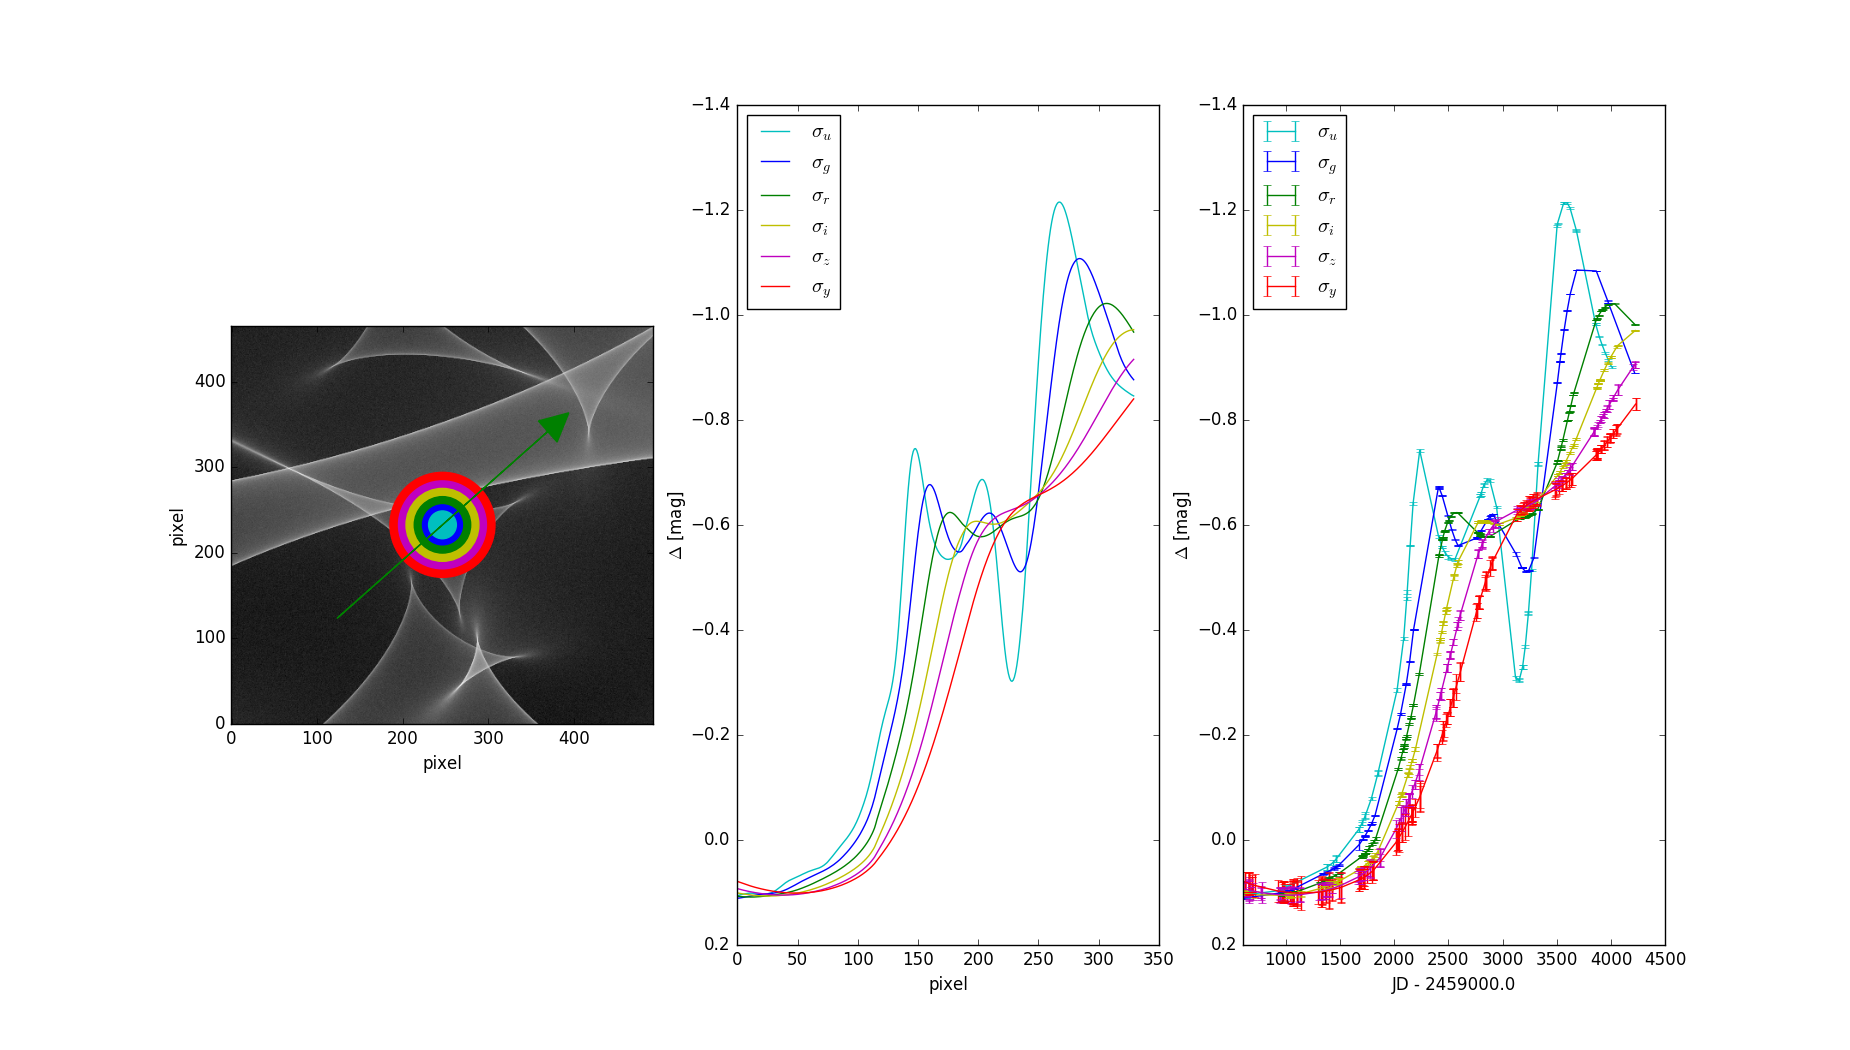
\includegraphics[width=\textwidth]{figs/agn/sim_ex.png}
		\caption{Ten year long simulated light curve for image A of RXJ1131-1231 using $\sigma_0$=2.0 light days at 2000\AA{}, $\alpha$=0.75, $\kappa$=0.494, $\gamma$=0.562 and 40\% of matter in compact form (stars). The left panel shows the concentric Gaussian emission regions observed by the LSST filters projected on top of the magnification pattern. The center panel shows the light curves with a ``perfect'' cadence. The right panel shows the magnitude values interpolated at epochs observed by LSST at the location of the system according the the ``Baseline Cadence'' (\opsimdbref{db:baseCadence})) Opsim output. The quasar was assumed to have the same intrinsic brightness in each band for easier comparison of variations between bands.}
		\label{microsimcurve}
	\end{figure}
\end{center}

% --------------------------------------------------------------------

\subsection{Metrics}
\label{sec:\secname:metrics}

Metrics for these section need to be defined by using simulated light curves
that take into account the several parameters that come into play in quasar
microlensing. These include: the time gap between visits in the same band,
projected CMB velocity, simulated peculiar velocities and redshifts of lenses
and sources as well as ``macro'' lens model parameters (i.e., surface mass
density and shear projected on top of lensed quasar images). Two metrics are
currently in consideration:

High Magnification Events recovery metric: This metric will measure the
number of high-magnification events recovered/missed considering the
cadence and season length in every LSST band and as the precision of the
brightness measurement.



Accretion disk size and slope metric: This metric will do a full
analysis of the ``pure'' microlensing light curves to recover these two
physical AGN parameters. The figure of merit would be the accuracy of
the measurement.

Since the microlensing signal can only be obtained after time delays between images
have been measured, both metrics need close interaction with time delay
measurements. As such, the ``Time Delays Challenges'' (see
\autoref{sec:lenstimedelays}) will include complete microlensing signal
simulations which also take into account the aforementioned parameters. Note
that given
the dependence on individual filter cadence and season length as well as
projected CMB velocities, every region on the sky needs to be considered
independently. Time Delay Challenge submissions will thus include recovered
``pure'' microlensing
light curves in addition to measured time-delays. By doing the reverse
procedure, i.e. using these ``pure'' microlensing light curves to statistically
re-obtain the input accretion disk sizes and thermal slopes, we will be able to
quantitatively measure the accuracy of the intrinsic accretion disk parameter
estimations for a given survey strategy.



We have build a preliminary tool that extracts micro lensing light curves from source plane magnification patterns as will be observed by LSST, taking into account:
\begin{itemize}
\item Projected peculiar velocities of the observer (projected CMB dipole in the direction of the system), lens and source.
\item Bulk motion of stars in the lensing galaxy (from the stellar velocity dispersion of the lens).
\item Specific LSST observing epochs in the direction of the system (from Opsim outputs).
\item Thermal profile slope of the accretion disk $\alpha$.
\item Scale size of the accretion disk $\sigma_{0}(\lambda)$ at a given wavelength $\lambda$.
\item Smooth (dark matter) to compact (stars) matter ratio on top of lensed quasar images.
\item ��Macro'' lens model parameters on top of lensed quasar images: Surface mass density $\kappa$ and shear $\gamma$.
\end{itemize}

\noindent In its current state, the tool assumes simple face-on concentric Gaussian emission regions for the accretion disk. An example of such a curve is shown in figure \ref{microsimcurve}. To recover the figure of merit, (measurement accuracy of $\alpha$ and $\sigma_0$), light curves generated with this tool for a given realistic lensed quasar system ($\kappa$, $\gamma$, s and velocity dispersion of the lensing galaxy as well as time delays between lensed images) for every region in the sky need to analyzed using the above mentioned statistical analyses to recover the input accretion disk parameters.


% microlensing - convolve microlensing timescales for QSOs we already know
% about. how many of the high magnification events do we get? How bright?
% @tanguita

% --------------------------------------------------------------------

\subsection{OpSim Analysis}
\label{sec:\secname:analysis}

Much like the cosmology with lensed quasar time delays, we expect a strong
dependence of the proposed metrics with night-to-night cadence, uniformity and
season length. Maximizing these will maximize the likelihood of recovering high
magnification events, which in turn will provide the most stringent constraints
on
accretion disk structure. As mentioned above, since shorter wavelengths show
faster and stronger magnification events, in an ideal scenario, bluer bands would have
tighter night-to-night cadence.

\begin{center}
	\begin{figure}[hbt]
		\includegraphics[width=\textwidth]{figs/agn/NightSep_seasonLength.pdf}
		\caption{Median Night Separation in days (left) and median season length in months (right) for all bands in the current ``Baseline Cadence'' (\opsimdbref{db:baseCadence}, top) and ``No Visit Pairs''	(\opsimdbref{db:NoVisitPairs}, bottom) opsim outputs.}
		\label{microfig}
	\end{figure}
\end{center}

As shown in figure \ref{microfig}, it seems there is a slightly better prospect
for the AGN structure with microlensing science case using the ``No Visit Pairs'' observing
strategy in comparison to the baseline strategy due to the smaller inter-night
gaps and longer season lengths in the g band. In both cases the night-to-night
cadence in the longer wavebands are compatible with the detection of most
microlensing events. On the other hand, in the u and g bands in both survey strategies it might compromise the results. Furthermore, in all LSST bands the spread in the night-to-night cadence (uniformity) and season length will likely dominate the uncertainties.

\begin{center}
	\begin{figure}[hbt]
		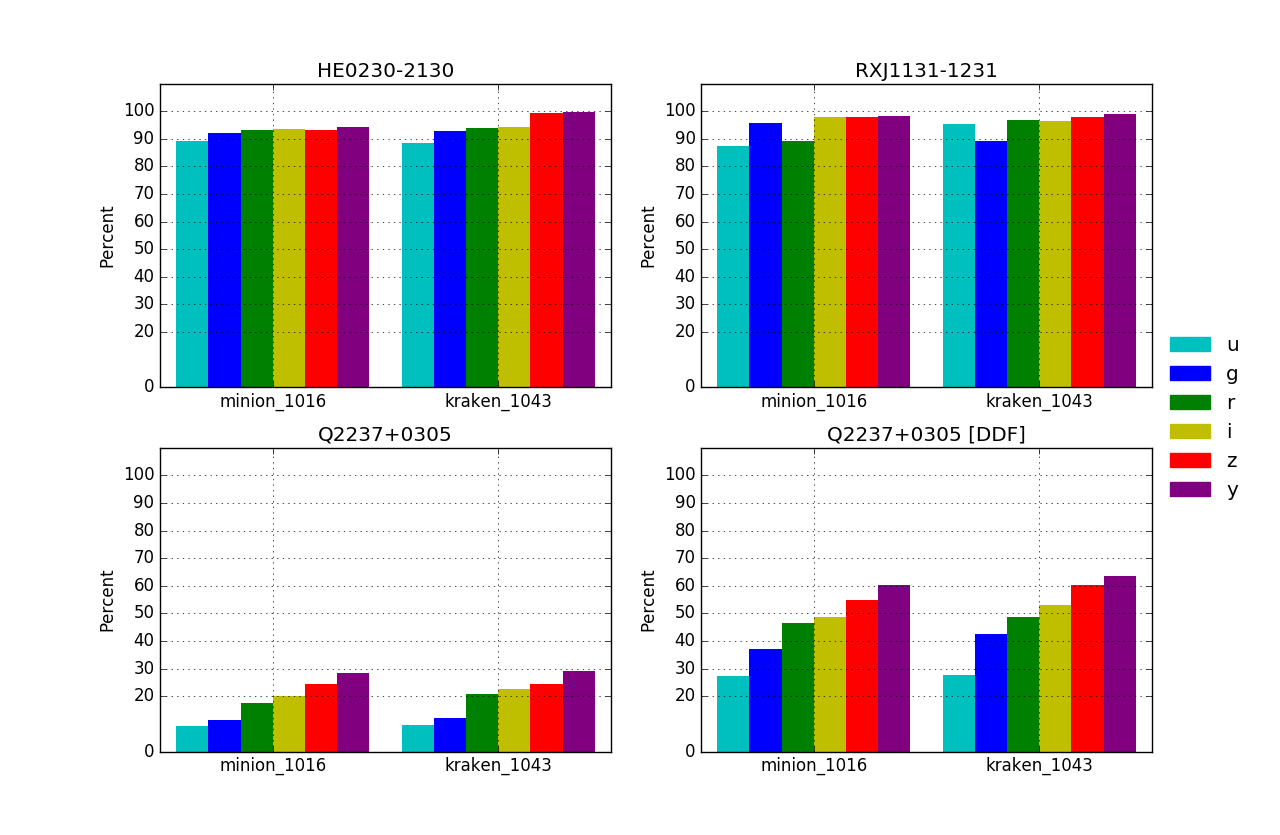
\includegraphics[width=\textwidth]{figs/agn/ulens_sim.png}
		\caption{Relative brightness fluctuations seen by LSST compared to ``perfect'' cadence for four systems as described in the text. The current ``Baseline Cadence'' (\opsimdbref{db:baseCadence}) and ``No Visit Pairs''	(\opsimdbref{db:NoVisitPairs}) opsim outputs are shown.All systems assumed to have accretion disk parameters of $\sigma_0$=2.0 light days and $\alpha$=0.75. Ratios are the median of 10000 simulated light curves.}
		\label{ulens_sim}
	\end{figure}
\end{center}


Given the nature of the commonly used statistical analyses to constrain the structure of accretion disk (accretion disk and slope metric), the accuracy of the recovery of the parameters will depend on the amount of brightness variations seen in the light curves even if no high-magnification events are seen. As a first assessment, we have used the light curve simulation tool outlined above to generate 10000 light curves for images A of three well known lensed systems where microlensing has been studied: RXJ1131-1231, HE0230-2130 and Q2237+0305. Additionally, given the very fast time scales expected for Q2237+0305 due to the relative redshifts of the source and lens, we also generate 10000 light curves for this system as if it was located in one of the LSST Deep Drilling Fields. All systems where assumed to have a size ($\sigma_0$) and slope ($\alpha$) parameters of 2.0 light days at $\lambda$=2000\AA{} and 0.75, respectively. Even when this experiment does not yield our proposed figure of merit, it does allow the comparison of the relative performance of different observing strategy regarding microlensing signal recovery.

The results of this experiment are shown in Figure \ref{ulens_sim}. For this analysis, at least for the four systems studied, we can see that even when the ``No Visit Pairs'' observing strategy shows a slightly better prospect compared to the ``Baseline Cadence'' for our science case, the difference is negligible. Note also that with the exception of Q2227+0305 (due to its very short time scales), both observing strategies will be able to map the expected microlensing induced brightness variations at a very high rate. It is important to consider that this is an optimistic analysis because the photometric uncertainties (including the dominating ones that come from the intrinsic variability correction from time delay measurements) have not been taken into account.


\subsection{Conclusions}
\label{sec:\secname:questions}

Here we answer the ten questions posed in
\autoref{sec:intro:evaluation:caseConclusions}:

\begin{description}

\item[Q1:] {\it Does the science case place any constraints on the
tradeoff between the sky coverage and coadded depth? For example, should
the sky coverage be maximized (to $\sim$30,000 deg$^2$, as e.g., in
Pan-STARRS) or the number of detected galaxies (the current baseline but
with 18,000 deg$^2$)?}

\item[A1:] Given that lensed quasars are rare, maximizing the area
coverage would increase the number of systems to study. Even if this
comes at a cadence cost given that in most cases the studied OpSim
experiments provide sufficient temporal constraints.

\item[Q2:] {\it Does the science case place any constraints on the
tradeoff between uniformity of sampling and frequency of  sampling? For
example, a rolling cadence can provide enhanced sample rates over a part
of the survey or the entire survey for a designated time at the cost of
reduced sample rate the rest of the time (while maintaining the nominal
total visit counts).}

\item[A2:] Given the long timescales of microlensing events and the inability of predicting high-magnification events, uniform sampling would be better.

\item[Q3:] {\it Does the science case place any constraints on the
tradeoff between the single-visit depth and the number of visits
(especially in the $u$-band where longer exposures would minimize the
impact of the readout noise)?}

\item[A3:] No.

\item[Q4:] {\it Does the science case place any constraints on the
Galactic plane coverage (spatial coverage, temporal sampling, visits per
band)?}

\item[A4:] Not really, however, minimizing the coverage of the Galactic would benefit all AGN science cases.

\item[Q5:] {\it Does the science case place any constraints on the
fraction of observing time allocated to each band?}

\item[A5:] Ideally, shorter wavelengths should get denser (uniform) sampling.

\item[Q6:] {\it Does the science case place any constraints on the
cadence for deep drilling fields?}

\item[A6:] As in the main survey, AGN microlesing would benefit if the deep drilling fields observations would span long timescales with uniform coverage.

\item[Q7:] {\it Assuming two visits per night, would the science case
benefit if they are obtained in the same band or not?}

\item[A7:] Not very important for our since case. Given a choice, different bands would be better.

\item[Q8:] {\it Will the case science benefit from a special cadence
prescription during commissioning or early in the survey, such as:
acquiring a full 10-year count of visits for a small area (either in all
the bands or in a  selected set); a greatly enhanced cadence for a small
area?}

\item[A8:] No.

\item[Q9:] {\it Does the science case place any constraints on the
sampling of observing conditions (e.g., seeing, dark sky, airmass),
possibly as a function of band, etc.?}

\item[A9:] Seeing and Airmass are directly related to the ability to
accurately separate the flux from possibly blended lensed images. As
with most transient science cases, excellent seeing images are required
as templates for image substraction.

\item[Q10:] {\it Does the case have science drivers that would require
real-time exposure time optimization to obtain nearly constant
single-visit limiting depth?}

\item[A10:] No.

\end{description}


% % --------------------------------------------------------------------
%
% \subsection{Discussion}
% \label{sec:\secname:discussion}
%
% %Discussion: what risks have been identified? What suggestions could be
% %made to improve this science project's figure of merit, and mitigate
% %the identified risks?
%
%
% ====================================================================

\navigationbar


% --------------------------------------------------------------------

% ====================================================================
%+
% SECTION:
%    AGN_Future_Work.tex
%
% CHAPTER:
%    agn.tex
%
% ELEVATOR PITCH:
%    Ideas for future metric investigation, with quantitaive analysis
%    still pending.
%-
% ====================================================================

\section{Future Work}\label{sec:AGNFuture}
\def\secname{\chpname:future}\label{sec:\secname}

In this section we provide a short compendium of science cases that
are either still being developed, or that are deserving of quantitative
MAF analysis at some point in the future.

% ====================================================================

%% ====================================================================
%+
% SECTION:
%    AGN_Clustering.tex
%
% CHAPTER:
%    agn.tex
%
% ELEVATOR PITCH:
%-
% ====================================================================

% \section{AGN Clustering}
\subsection{AGN Clustering}\lebel{sec:AGNClustering}
\def\secname{\chpname:clustering}\label{sec:\secname}

\credit{ohadshemmer}

Measurements of the spatial clustering of AGNs with respect
to those of quiescent galaxies can provide clues as to how galaxies
form inside their dark-matter halos, and what causes the growth of
their supermassive black holes (SMBHs). The impressive inventory of
LSST AGNs will enable the clustering, and thus the host galaxy halo
mass, to be determined over the widest ranges of cosmic epoch
and accretion power.


% % --------------------------------------------------------------------
%
% \subsection{Target measurements and discoveries}
% \label{sec:\secname:targets}

% Describe the discoveries and measurements you want to make.

% Now, describe their response to the observing strategy. Qualitatively,
% how will the science project be affected by the observing schedule and
% conditions? In broad terms, how would we expect the observing strategy
% to be optimized for this science?

We would consider the 2-point angular correlation function of AGN as our
target measurement.
The LSST cadence will not only affect the overall AGN census and its
$L-z$ distribution, but also the depth in each band as a function of
sky position that can directly affect the clustering signal.

% CROSS REFERENCE TO THE COSMOLOGY CHAPTER'S LSS SECTION! WHAT'S
% DIFFERENT ABOUT AGN CLUSTERING?

% --------------------------------------------------------------------
%
% \subsection{Metrics}
% \label{sec:\secname:metrics}
%
% Quantifying the response via MAF metrics: definition of the metrics,
% and any derived overall figure of merit.
%
%
% % --------------------------------------------------------------------
%
% \subsection{OpSim Analysis}
% \label{sec:\secname:analysis}
%
% OpSim analysis: how good would the default observing strategy be, at
% the time of writing for this science project?
%
%
% % --------------------------------------------------------------------
%
% \subsection{Discussion}
% \label{sec:\secname:discussion}
%
% Discussion: what risks have been identified? What suggestions could be
% made to improve this science project's figure of merit, and mitigate
% the identified risks?
%
%
% ====================================================================
%
% \subsection{Conclusions}
%
% Here we answer the ten questions posed in
% \autoref{sec:intro:evaluation:caseConclusions}:
%
% \begin{description}
%
% \item[Q1:] {\it Does the science case place any constraints on the
% tradeoff between the sky coverage and coadded depth? For example, should
% the sky coverage be maximized (to $\sim$30,000 deg$^2$, as e.g., in
% Pan-STARRS) or the number of detected galaxies (the current baseline but
% with 18,000 deg$^2$)?}
%
% \item[A1:] ...
%
% \item[Q2:] {\it Does the science case place any constraints on the
% tradeoff between uniformity of sampling and frequency of  sampling? For
% example, a rolling cadence can provide enhanced sample rates over a part
% of the survey or the entire survey for a designated time at the cost of
% reduced sample rate the rest of the time (while maintaining the nominal
% total visit counts).}
%
% \item[A2:] ...
%
% \item[Q3:] {\it Does the science case place any constraints on the
% tradeoff between the single-visit depth and the number of visits
% (especially in the $u$-band where longer exposures would minimize the
% impact of the readout noise)?}
%
% \item[A3:] ...
%
% \item[Q4:] {\it Does the science case place any constraints on the
% Galactic plane coverage (spatial coverage, temporal sampling, visits per
% band)?}
%
% \item[A4:] ...
%
% \item[Q5:] {\it Does the science case place any constraints on the
% fraction of observing time allocated to each band?}
%
% \item[A5:] ...
%
% \item[Q6:] {\it Does the science case place any constraints on the
% cadence for deep drilling fields?}
%
% \item[A6:] ...
%
% \item[Q7:] {\it Assuming two visits per night, would the science case
% benefit if they are obtained in the same band or not?}
%
% \item[A7:] ...
%
% \item[Q8:] {\it Will the case science benefit from a special cadence
% prescription during commissioning or early in the survey, such as:
% acquiring a full 10-year count of visits for a small area (either in all
% the bands or in a  selected set); a greatly enhanced cadence for a small
% area?}
%
% \item[A8:] ...
%
% \item[Q9:] {\it Does the science case place any constraints on the
% sampling of observing conditions (e.g., seeing, dark sky, airmass),
% possibly as a function of band, etc.?}
%
% \item[A9:] ...
%
% \item[Q10:] {\it Does the case have science drivers that would require
% real-time exposure time optimization to obtain nearly constant
% single-visit limiting depth?}
%
% \item[A10:] ...
%
% \end{description}

% ====================================================================

\navigationbar


% --------------------------------------------------------------------

% ====================================================================
%+
% SECTION:
%    AGN_BELR.tex
%
% CHAPTER:
%    agn.tex
%
% ELEVATOR PITCH:
%
%-
% ====================================================================

% \section{The Size and Structure of the Broad Emission Line Region}
\subsection{The Size and Structure of the Broad Emission Line Region}\label{sec:AGNBELR}
\def\secname{\chpname:photoRM}\label{sec:\secname}

\credit{ohadshemmer}

LSST may provide estimates of the size and structure of the broad
emission line region (BELR) using the photometric reverberation
mapping (PRM) method. This method enables one to measure the
time-delayed response of the flux in one band to the flux
in another by using cross-correlation techniques on AGN light
curves (e.g.,
%\citet{Chelouche2013}; \citet{CheloucheandZucker2013};
\citealt{CheloucheEtal2014}).



%; \citet{EdelsonEtal2015}; \citet{FausnaughEtal2015}).
The main challenge of PRM is to detect,
with high confidence, the time lag between the variations of a BELR
line-rich band with respect to variations in a line-poor band, given
the relatively small flux contributions ($\sim10$\%)~of BELR lines to each
LSST band. Nevertheless, LSST is expected to deliver BELR line-continuum
time delays in $\sim10^5-10^6$ sources, which is unprecedented when
compared to $\sim60-80$ such measurements conducted, to date, via the
traditional, yet much more expensive (per source) spectroscopic method.
Sources in the DDFs will benefit from the highest
quality PRM time-delay measurements given the factor of $\sim10$ denser
sampling \citep{CheloucheEtal2014}.

% --------------------------------------------------------------------

% \subsection{Target measurements and discoveries}
\subsubsection{Target measurements and discoveries}
\label{sec:\secname:targets}

The PRM measurements will probe the size and structure of the BELR,
in a statistical sense, and may provide improved SMBH mass estimates
for sources that have at least single-epoch spectra. PRM will also be
used to trigger follow-up spectrophotometric monitoring of ``promising''
cases depending on their variability properties. The goal is to obtain
$R_{\rm BELR}$ measures for different BELR lines in certain luminosity
and redshift bins; for example, PRM may provide mean $R_{\rm BELR}$ for
Ly$\alpha$ in quasars at $2.1\ltsim z \ltsim 2.2$ with
$45 \ltsim \log L ({\rm erg~s}^{-1}) \ltsim 46$, or mean $R_{\rm BELR}$
for C~{\sc iv}~$\lambda 1549$ in quasars at $1.6\ltsim z \ltsim 1.7$
with $44 \ltsim \log L ({\rm erg~s}^{-1}) \ltsim 45$.
%\new{Our goal is to understand the population of
%AGN broad line regions, including their geometry. We expect to do this
%via  a model that connects the BH mass, BLR geometry and AGN
%photometric variability properties via a set of scaling relations. A
%simple version of this is could be something like...\newline\newline
%So, our target measurements are of $a$ and $b$, the X parameters.
%Before we derive a metric that quantifies our ability to measure these
%parameters, we can anticipate some of the sensitivity of the
%photometric RM method to observing strategy.}

The PRM method is very sensitive to the sampling in each band,
therefore the ability to derive reliable time delays can be affected
significantly by the LSST cadence. The best results will be obtained
by having the most uniform sampling equally for each band.
%
Since the observed line-continuum lags scale with luminosity and redshift,
PRM with the LSST will be limited by the average time gaps between successive
observations in a particular band.
%
Additionally, there is a trade-off between the number of DDFs and the
number of time delays that PRM can obtain \citep{CheloucheEtal2014}.
For example, an increase in the number of DDFs, with similarly dense
sampling in each field, can yield a proportionately larger number of
high-quality time delays, down to somewhat lower luminosities (to the
extent that host-galaxy contamination can be neglected), but at the
expense of far fewer time delays (for relatively high luminosity
sources) in the main survey.

% --------------------------------------------------------------------

% \subsection{Metrics}
\subsubsection{Metrics}
\label{sec:\secname:metrics}

The average and the dispersion in the number of visits, per band, across
the sky for the nominal OpSim (during the entire survey) should be computed.
Since PRM works best for uniform sampling, one should compare the distributions
of the number of visits in each band, averaged across the sky, and identify
ways to minimize any potential differences between these distributions. By
running PRM simulations, one should identify the 1) minimum number of visits
(in any band) that can yield any meaningful BELR-continuum lag estimates, and
2) the largest difference in the number of visits between two different bands
that can yield any meaningful BELR-continuum lag estimates. These simulations
should be repeated by doubling the nominal number of DDFs. Finally, the
%number of meaningful BELR-continuum time delays that can be obtained
uncertainties on $R_{\rm BELR}$ values achieved with the nominal OpSim
should be assessed, and potential perturbations to the cadence should be
pointed out to reduce these uncertainties.

Another metric is the accuracy of the slope $\alpha$, $\Delta \alpha$, in the
$R_{\rm BELR} \propto L^{\alpha}$ relation. Spectrophotometric monitoring
typically yields $\alpha \simeq 0.50 \pm 0.05$.

% % --------------------------------------------------------------------
%
% \subsection{OpSim Analysis}
% \label{sec:\secname:analysis}
%
% OpSim analysis: how good would the default observing strategy be, at
% the time of writing for this science project?
%
%
% % --------------------------------------------------------------------
%
% \subsection{Discussion}
% \label{sec:\secname:discussion}
%
% Discussion: what risks have been identified? What suggestions could be
% made to improve this science project's figure of merit, and mitigate
% the identified risks?
%
%
% ====================================================================
%
% \subsection{Conclusions}
%
% Here we answer the ten questions posed in
% \autoref{sec:intro:evaluation:caseConclusions}:
%
% \begin{description}
%
% \item[Q1:] {\it Does the science case place any constraints on the
% tradeoff between the sky coverage and coadded depth? For example, should
% the sky coverage be maximized (to $\sim$30,000 deg$^2$, as e.g., in
% Pan-STARRS) or the number of detected galaxies (the current baseline but
% with 18,000 deg$^2$)?}
%
% \item[A1:] ...
%
% \item[Q2:] {\it Does the science case place any constraints on the
% tradeoff between uniformity of sampling and frequency of  sampling? For
% example, a rolling cadence can provide enhanced sample rates over a part
% of the survey or the entire survey for a designated time at the cost of
% reduced sample rate the rest of the time (while maintaining the nominal
% total visit counts).}
%
% \item[A2:] ...
%
% \item[Q3:] {\it Does the science case place any constraints on the
% tradeoff between the single-visit depth and the number of visits
% (especially in the $u$-band where longer exposures would minimize the
% impact of the readout noise)?}
%
% \item[A3:] ...
%
% \item[Q4:] {\it Does the science case place any constraints on the
% Galactic plane coverage (spatial coverage, temporal sampling, visits per
% band)?}
%
% \item[A4:] ...
%
% \item[Q5:] {\it Does the science case place any constraints on the
% fraction of observing time allocated to each band?}
%
% \item[A5:] ...
%
% \item[Q6:] {\it Does the science case place any constraints on the
% cadence for deep drilling fields?}
%
% \item[A6:] ...
%
% \item[Q7:] {\it Assuming two visits per night, would the science case
% benefit if they are obtained in the same band or not?}
%
% \item[A7:] ...
%
% \item[Q8:] {\it Will the case science benefit from a special cadence
% prescription during commissioning or early in the survey, such as:
% acquiring a full 10-year count of visits for a small area (either in all
% the bands or in a  selected set); a greatly enhanced cadence for a small
% area?}
%
% \item[A8:] ...
%
% \item[Q9:] {\it Does the science case place any constraints on the
% sampling of observing conditions (e.g., seeing, dark sky, airmass),
% possibly as a function of band, etc.?}
%
% \item[A9:] ...
%
% \item[Q10:] {\it Does the case have science drivers that would require
% real-time exposure time optimization to obtain nearly constant
% single-visit limiting depth?}
%
% \item[A10:] ...
%
% \end{description}

% ====================================================================

\navigationbar


% ====================================================================


% --------------------------------------------------------------------

\section{Discussion}\label{sec:AGNDiscussion}
\label{sec:\chpname:discussion}

%Some additional considerations/thoughts that came up during the Bremerton
%workshop:

The goals of this Chapter were 1) to define and quantify key metrics for AGN
science that can be measured and tested using the current LSST observing
strategy, and 2) to identify reasonable perturbations that may be beneficial
for AGN science.
%
Undoubtedly, additional work is required to refine many of these metrics
and perform more rigorous tests and simulations.
%
The following list identifies additional cadence-related aspects for further
consideration. Together with the metrics discussed in this Chapter, this may
be regarded as a road map for further investigations that should be performed
during the planning stage.

1) Assuming a total of ten DDFs, it would be beneficial if one of those fields
could be sampled more heavily than the others and would be visited nightly (or
even more frequently, e.g., from $\sim1$ to $\sim1000$ min) per band.
This can be justified by the fact that a) very few AGNs or transient AGNs have
been monitored at these frequencies on such a long baseline, leaving room for
discovery, and b) this may probe intermediate-mass black holes
($\sim10^4 - 10^5$~$M_{\odot}$) via PRM or PSDs. Good candidate fields are
the Magellanic Clouds and the Chandra Deep Field-South. An observational
strategy should be developed and implemented either in a new OpSim, or
during commissioning.

%2) An assessment of the effects of the LSST cadence on the ability to
%detect periodic AGNs and quasi-periodic oscillations (QPOs) in AGNs
%should be performed.

2) In order to have more informative metrics, accurate model light
curves are needed that can reproduce fiducial light curves in different
bands, at different inherent luminosities, and at different redshifts.
This may be developed together with the Strong Lensing Science Collaboration.

% DDF - we need longer duration OpSims in these fields. (Bob Wagoner)
% (https://github.com/LSSTScienceCollaborations/ObservingStrategy/blob/master/opsim/README.md)

% commissioning opportunity - one field, one night, one filter (u or g).
% 15/30 sec exposures. (Bob Wagoner)
% (https://github.com/LSSTScienceCollaborations/ObservingStrategy/blob/master/commissioning/README.md)

%\todo{}{
3) There is a need to compare the science content in this Chapter
with the AGN chapter in the LSST Science Book as well as with the
Ivezic et al. overview paper (http://arxiv.org/pdf/0805.2366v4.pdf)
to ensure that no key science aspect is overlooked or compromised
by the nominal cadence.
%}

%\todo{}{Compare the $Y$-band (and other bands) depths, single
%epoch and final co-added, from  enigma\_1189 with other OpSims.}

%\todo{}{Assess the effect of non-simultaneous colors on AGN selection.}

%\todo{}{Based on the current OpSim, need to specify the magnitude limits
%at the highest airmass and assess the limitations of the DCR method in
%the $L-z$ plane. Should check this with MAF and if indeed AM <= 1.4, need
%to add a request in:
%https://github.com/LSSTScienceCollaborations/ObservingStrategy/tree/master/opsim
%}

%\todo{}{Assess whether, e.g., a pair of $\sim2.5$ min exposures (i.e., $\sim10$
%times longer than the standard exposures) at airmass $\sim2$ would get deep
%enough for useful DCR constraints for a large fraction of the AGNs. This may
%be a non-negligible perturbation of the expected 56-184 visits per band, and
%may even be impossible given current upper limits on exposure times, but
%this would help improve photo-z's for galaxies and SNe too.}

%\todo{}{For PRM and microlensing: obtain distributions (mean and dispersion)
%of the number of visits, per band, across the sky for the nominal OpSim
%(during the entire survey).}

%\todo{}{
4) It is worth checking whether
%Add a discussion about blazars and LSST cadence (e.g., Isler+15?). Would
any aspect of blazar science might be compromised by the nominal cadence, or
would benefit from a specific cadence requirement.
%}

%\todo{}{
5) The effects of the cadence on the overall LSST astrometry accuracy and precision
should be assessed in terms of potential effects on AGN selection. For example,
AGN selection may benefit from very good depth at least in the 1st and 10th year of the
survey.
%}

%\todo{}{
%6) It is necessary to identify the frequency range and sampling for obtaining
%optimal PSDs required for QPO detection (given $M_{\rm BH}$, spin, and $L/L_{\rm Edd}$).
%Based on the nominal cadence, it is necessary to assess the potential of discovering
%QPOs in the main survey and in the DDFs.
%}

\navigationbar
